\documentclass{whiteboard}
\begin{document}
\begin{frame}[plain,t]
\bbcover{OJ 10171}{Meeting Prof. Miguel...}{Prof. Edson Alves}{Faculdade UnB Gama}

\end{frame}
\begin{frame}[plain,t]
\vspace*{\fill}

\bbenglish{I have always thought that someday I will meet Professor Miguel, who has allowed me to arrange so many contests. But I have managed to miss all the opportunities in reality. At last with the help of a magician I have managed to meet him in the magical \bbbold{City of Hope}. The city of hope has many roads. Some of them are bi-directional and others are unidirectional. Another important property of these streets are that some of the streets are for people whose age is less than thirty and rest are for the others. This is to give the minors freedom in their activities.  Each street has a certain length. Given the description of such a city and our initial positions, you will have to find the most suitable place where we can meet. The most suitable place is the place where our combined effort of reaching is minimum. You can assume that I am 25 years old and Prof. Miguel is 40+.}

\vspace*{\fill}
\end{frame}
\begin{frame}[plain,t]
\vspace*{\fill}

\bbtext{Eu sempre pensei que algum dia eu iria me encontrar com o Professor Miguel, que tem me permitido preparar muitos eventos. Mas, de fato, eu perdi todas as oportunidades. Enfim, com a ajuda de um mágico eu consegui encontrá-lo na mágica \bbbold{Cidade da Esperança}. A cidade da esperança tem muitas ruas. Algumas delas são bidirecionais, outras unidirecionais. Outra propriedade importante destas ruas é que algumas delas são para pessoas com menos do que 30 anos e as outras são para os demais cidadãos. Isto é feito para dar aos menores liberdade em suas atividades.  Cada rua tem um certo comprimento. Dada a descrição de cada cidade e as nossas posições iniciais, determine o local mais apropriado para o encontro. O lugar mais apropriado é o lugar cujo esforço combinado de ambos para chegar lá é minimo. Você pode assumir que eu tenho 25 anos e o Prof. Miguel tem 40 ou mais.}

\vspace*{\fill}
\end{frame}
\begin{frame}[plain,t]
\vspace*{\fill}

\begin{figure}
\includegraphics[scale=1.3]{figs/figure.png}
\caption{\bbenglish{Shahriar Manzoor and Miguel A.  Revilla (Shanghai, 2005).  First meeting after five years of collaboration}}
\end{figure}

\vspace*{\fill}
\end{frame}
\begin{frame}[plain,t]
\vspace*{\fill}

\begin{figure}
\includegraphics[scale=1.3]{figs/figure.png}
\caption{\bbtext{Shahriar Manzoor e Miguel A.  Revilla (Shanghai, 2005).  Primeiro encontro após cinco anos de colaboração}}
\end{figure}

\vspace*{\fill}
\end{frame}
\begin{frame}[plain,t]
\vspace*{\fill}

\bbbold{Input}

\vspace{0.1in}

\bbenglish{The input contains several descriptions of cities. Each description of city is started by a integer $N$, which indicates how many streets are there. The next $N$ lines contain the description of $N$ streets.}

\vspace{0.1in}

\bbenglish{The description of each street consists of four uppercase alphabets and an integer. The first alphabet is either ‘\texttt{Y}’ (indicates that the street is for young) or ‘\texttt{M}’ (indicates that the road is for people aged 30 or more) and the second character is either ‘\texttt{U}’ (indicates that the street is unidirectional) or ‘\texttt{B}’ (indicates that the street is bi-directional). The third and fourth characters, $X$ and $Y$ can be any uppercase alphabet and they indicate that place named $X$ and $Y$ of the city are connected (in case of unidirectional it means that there is a one-way street from $X$ to $Y$) and the last non-negative integer $C$ indicates the energy required to walk through the street. If we are in the same place we can meet each other in zero cost anyhow. Every energy value is less than $500$.}

\vspace*{\fill}
\end{frame}
\begin{frame}[plain,t]
\vspace*{\fill}

\bbbold{Input}

\vspace{0.1in}

\bbtext{A entrada contém várias descrições de cidades. Cada descrição de cidade começa com um inteiro $N$, o qual indica quantas ruas há na cidade. As próximas $N$ linhas contém as descrições das $N$ ruas.}

\vspace{0.1in}

\bbtext{A descrição de cada rua consiste em quatro letras maiúsculas do alfabeto e um inteiro. A primeira letra é ou ‘\texttt{Y}’ (indicando que a rua é para os jovens) ou ‘\texttt{M}’ (indicando que a rua é para pessoas com 30 anos ou mais) e o segundo caractere ou é ‘\texttt{U}’ (indicando que a rua é unidirecional) ou ‘\texttt{B}’ (indicando que a rua é bidirecional). O terceiro e o quarto caracteres $X$ e $Y$ podem ser qualquer letra maiúscula do alfabeto e indicam que os lugares $X$ e $Y$ da cidade estão conectados (no caso unidirecional significa que há uma rua de mão única com sentido de $X$ a $Y$) e o inteiro não-negativo $C$ indica que a energia necessária para caminhar pela rua. Se ambos estamos no mesmo lugar nós podemos nos encontrar com custo zero, de algum modo. Os valores da energia são menores do que $500$.}


\vspace*{\fill}
\end{frame}
\begin{frame}[plain,t]
\vspace*{\fill}

\bbenglish{After the description of the city the last line of each input contains two place names, which are the initial position of me and Prof. Miguel respectively.}

\vspace{0.1in}

\bbenglish{A value zero for $N$ indicates end of input.}

\vspace{0.2in}

\bbbold{Output}

\vspace{0.1in}

\bbenglish{For each set of input, print the minimum energy cost and the place, which is most suitable for us to meet. If there is more than one place to meet print all of them in lexicographical order in the same line, separated by a single space. If there is no such places where we can meet then print the line ‘\texttt{You will never meet.}’}

\vspace*{\fill}
\end{frame}
\begin{frame}[plain,t]
\vspace*{\fill}

\bbtext{Após a descrição de uma cidade a última linha de cada entrada contém o nome de dois lugares, os quais são as posições iniciais onde estão eu e o prof. Miguel, respectivamente.}

\vspace{0.1in}

\bbtext{O valor $N$ igual a zero indica o fim da entrada.}

\vspace{0.2in}

\bbbold{Saída}

\vspace{0.1in}

\bbtext{Para cada conjunto da entrada, imprima o custo mínimo de energia necessário e o lugar mais apropriado para o encontro. Se existe mais de um lugar imprima todos eles, em ordem lexicográfica, na mesma linha, separados por um único espaço em branco. Se não há um lugar apropriado para o encontro imprima a mensagem ‘\texttt{You will never meet.}’}

\vspace*{\fill}
\end{frame}
\begin{frame}[plain,t]
\begin{tikzpicture}
\node[draw,opacity=0] at (0, 0) {x};
\node[draw,opacity=0] at (14, 8) {x};

	\node[anchor=west] (header) at (0, 7.0) { \bbbold{Exemplo de entrada e saída} };

\end{tikzpicture}
\end{frame}
\begin{frame}[plain,t]
\begin{tikzpicture}
\node[draw,opacity=0] at (0, 0) {x};
\node[draw,opacity=0] at (14, 8) {x};

	\node[anchor=west] (header) at (0, 7.0) { \bbbold{Exemplo de entrada e saída} };


	\node[anchor=west] (line1) at (1.0, 6.0) { \bbtext{\texttt{2} } };

\end{tikzpicture}
\end{frame}
\begin{frame}[plain,t]
\begin{tikzpicture}
\node[draw,opacity=0] at (0, 0) {x};
\node[draw,opacity=0] at (14, 8) {x};

	\node[anchor=west] (header) at (0, 7.0) { \bbbold{Exemplo de entrada e saída} };


	\node[anchor=west] (line1) at (1.0, 6.0) { \bbtext{\texttt{2} } };


	\draw[->,color=BBViolet] (1.25, 5.0) to  (1.25, 5.75);

	\node[] (r) at (1.25, 4.75) { \footnotesize \bbcomment{\# de vértices} };

\end{tikzpicture}
\end{frame}
\begin{frame}[plain,t]
\begin{tikzpicture}
\node[draw,opacity=0] at (0, 0) {x};
\node[draw,opacity=0] at (14, 8) {x};

	\node[anchor=west] (header) at (0, 7.0) { \bbbold{Exemplo de entrada e saída} };


	\node[anchor=west] (line1) at (1.0, 6.0) { \bbtext{\texttt{2} } };





	\node[draw,very thick,circle] (node1) at (7.0, 4.0) { \bbtext{1} };

	\node[draw,very thick,circle] (node2) at (12.0, 4.0) { \bbtext{2} };

\end{tikzpicture}
\end{frame}
\begin{frame}[plain,t]
\begin{tikzpicture}
\node[draw,opacity=0] at (0, 0) {x};
\node[draw,opacity=0] at (14, 8) {x};

	\node[anchor=west] (header) at (0, 7.0) { \bbbold{Exemplo de entrada e saída} };


	\node[anchor=west] (line1) at (1.0, 6.0) { \bbtext{\texttt{2} } };





	\node[draw,very thick,circle] (node1) at (7.0, 4.0) { \bbtext{1} };

	\node[draw,very thick,circle] (node2) at (12.0, 4.0) { \bbtext{2} };


	\node[anchor=west] (line2) at (1.0, 5.5) { \bbtext{\texttt{0 5} } };

	\node[anchor=west] (line3) at (1.0, 5.0) { \bbtext{\texttt{4 0} } };

\end{tikzpicture}
\end{frame}
\begin{frame}[plain,t]
\begin{tikzpicture}
\node[draw,opacity=0] at (0, 0) {x};
\node[draw,opacity=0] at (14, 8) {x};

	\node[anchor=west] (header) at (0, 7.0) { \bbbold{Exemplo de entrada e saída} };


	\node[anchor=west] (line1) at (1.0, 6.0) { \bbtext{\texttt{2} } };


	\draw[->,color=BBViolet] (1.45, 3.75) to  (1.45, 4.75);

	\node[] (r) at (1.85, 3.5) { \bbcomment{matriz de adjacências} };


	\node[draw,very thick,circle] (node1) at (7.0, 4.0) { \bbtext{1} };

	\node[draw,very thick,circle] (node2) at (12.0, 4.0) { \bbtext{2} };


	\node[anchor=west] (line2) at (1.0, 5.5) { \bbtext{\texttt{0 5} } };

	\node[anchor=west] (line3) at (1.0, 5.0) { \bbtext{\texttt{4 0} } };



\end{tikzpicture}
\end{frame}
\begin{frame}[plain,t]
\begin{tikzpicture}
\node[draw,opacity=0] at (0, 0) {x};
\node[draw,opacity=0] at (14, 8) {x};

	\node[anchor=west] (header) at (0, 7.0) { \bbbold{Exemplo de entrada e saída} };


	\node[anchor=west] (line1) at (1.0, 6.0) { \bbtext{\texttt{2} } };





	\node[draw,very thick,circle] (node1) at (7.0, 4.0) { \bbtext{1} };

	\node[draw,very thick,circle] (node2) at (12.0, 4.0) { \bbtext{2} };


	\node[anchor=west] (line2) at (1.0, 5.5) { \bbtext{\texttt{0 5} } };

	\node[anchor=west] (line3) at (1.0, 5.0) { \bbtext{\texttt{4 0} } };




	\draw[very thick,-latex](node1) to [bend left] node[above] { \bbinfo{5} } (node2);

	\draw[very thick,-latex](node2) to [bend left] node[above] { \bbinfo{4} } (node1);

\end{tikzpicture}
\end{frame}
\begin{frame}[plain,t]
\begin{tikzpicture}
\node[draw,opacity=0] at (0, 0) {x};
\node[draw,opacity=0] at (14, 8) {x};

	\node[anchor=west] (header) at (0, 7.0) { \bbbold{Exemplo de entrada e saída} };


	\node[anchor=west] (line1) at (1.0, 6.0) { \bbtext{\texttt{2} } };





	\node[draw,very thick,circle] (node1) at (7.0, 4.0) { \bbtext{1} };

	\node[draw,very thick,circle] (node2) at (12.0, 4.0) { \bbtext{2} };


	\node[anchor=west] (line2) at (1.0, 5.5) { \bbtext{\texttt{0 5} } };

	\node[anchor=west] (line3) at (1.0, 5.0) { \bbtext{\texttt{4 0} } };




	\draw[very thick,-latex](node1) to [bend left] node[above] { \bbinfo{5} } (node2);

	\draw[very thick,-latex](node2) to [bend left] node[above] { \bbinfo{4} } (node1);


	\node[anchor=west] (line4) at (1.0, 4.5) { \bbtext{\texttt{1 2} } };

\end{tikzpicture}
\end{frame}
\begin{frame}[plain,t]
\begin{tikzpicture}
\node[draw,opacity=0] at (0, 0) {x};
\node[draw,opacity=0] at (14, 8) {x};

	\node[anchor=west] (header) at (0, 7.0) { \bbbold{Exemplo de entrada e saída} };


	\node[anchor=west] (line1) at (1.0, 6.0) { \bbtext{\texttt{2} } };


	\draw[->,color=BBViolet] (1.45, 3.25) to  (1.45, 4.25);

	\node[] (r) at (1.85, 3.0) { \bbcomment{vértices excluídos} };


	\node[draw,very thick,circle] (node1) at (7.0, 4.0) { \bbtext{1} };

	\node[draw,very thick,circle] (node2) at (12.0, 4.0) { \bbtext{2} };


	\node[anchor=west] (line2) at (1.0, 5.5) { \bbtext{\texttt{0 5} } };

	\node[anchor=west] (line3) at (1.0, 5.0) { \bbtext{\texttt{4 0} } };




	\draw[very thick,-latex](node1) to [bend left] node[above] { \bbinfo{5} } (node2);

	\draw[very thick,-latex](node2) to [bend left] node[above] { \bbinfo{4} } (node1);


	\node[anchor=west] (line4) at (1.0, 4.5) { \bbtext{\texttt{1 2} } };




\end{tikzpicture}
\end{frame}
\begin{frame}[plain,t]
\begin{tikzpicture}
\node[draw,opacity=0] at (0, 0) {x};
\node[draw,opacity=0] at (14, 8) {x};

	\node[anchor=west] (header) at (0, 7.0) { \bbbold{Exemplo de entrada e saída} };


	\node[anchor=west] (line1) at (1.0, 6.0) { \bbtext{\texttt{2} } };





	\node[draw,very thick,circle] (node1) at (7.0, 4.0) { \bbtext{1} };

	\node[draw,very thick,circle] (node2) at (12.0, 4.0) { \bbtext{2} };


	\node[anchor=west] (line2) at (1.0, 5.5) { \bbtext{\texttt{0 5} } };

	\node[anchor=west] (line3) at (1.0, 5.0) { \bbtext{\texttt{4 0} } };




	\draw[very thick,-latex](node1) to [bend left] node[above] { \bbinfo{5} } (node2);

	\draw[very thick,-latex](node2) to [bend left] node[above] { \bbinfo{4} } (node1);


	\node[anchor=west] (line4) at (1.0, 4.5) { \bbtext{\texttt{1 2} } };





	\node[] (eq) at (7.0, 1.5) { $\displaystyle \sum_{u, v, u\neq v} d(1, u, v) = d(1, 1, 2) + d(1, 2, 1) = 5 + 4 = 9$ };

\end{tikzpicture}
\end{frame}
\begin{frame}[plain,t]
\begin{tikzpicture}
\node[draw,opacity=0] at (0, 0) {x};
\node[draw,opacity=0] at (14, 8) {x};

	\node[anchor=west] (header) at (0, 7.0) { \bbbold{Exemplo de entrada e saída} };


	\node[anchor=west] (line1) at (1.0, 6.0) { \bbtext{\texttt{2} } };





	\node[draw,very thick,circle,fill=BBRed] (node1) at (7.0, 4.0) { \bbtext{1} };

	\node[draw,very thick,circle] (node2) at (12.0, 4.0) { \bbtext{2} };


	\node[anchor=west] (line2) at (1.0, 5.5) { \bbtext{\texttt{0 5} } };

	\node[anchor=west] (line3) at (1.0, 5.0) { \bbtext{\texttt{4 0} } };




	\draw[very thick,-latex](node1) to [bend left] node[above] { \bbinfo{5} } (node2);

	\draw[very thick,-latex](node2) to [bend left] node[above] { \bbinfo{4} } (node1);


	\node[anchor=west] (line4) at (1.0, 4.5) { \bbtext{\texttt{1 2} } };








\end{tikzpicture}
\end{frame}
\begin{frame}[plain,t]
\begin{tikzpicture}
\node[draw,opacity=0] at (0, 0) {x};
\node[draw,opacity=0] at (14, 8) {x};

	\node[anchor=west] (header) at (0, 7.0) { \bbbold{Exemplo de entrada e saída} };


	\node[anchor=west] (line1) at (1.0, 6.0) { \bbtext{\texttt{2} } };






	\node[draw,very thick,circle] (node2) at (12.0, 4.0) { \bbtext{2} };


	\node[anchor=west] (line2) at (1.0, 5.5) { \bbtext{\texttt{0 5} } };

	\node[anchor=west] (line3) at (1.0, 5.0) { \bbtext{\texttt{4 0} } };







	\node[anchor=west] (line4) at (1.0, 4.5) { \bbtext{\texttt{1 2} } };










\end{tikzpicture}
\end{frame}
\begin{frame}[plain,t]
\begin{tikzpicture}
\node[draw,opacity=0] at (0, 0) {x};
\node[draw,opacity=0] at (14, 8) {x};

	\node[anchor=west] (header) at (0, 7.0) { \bbbold{Exemplo de entrada e saída} };


	\node[anchor=west] (line1) at (1.0, 6.0) { \bbtext{\texttt{2} } };






	\node[draw,very thick,circle] (node2) at (12.0, 4.0) { \bbtext{2} };


	\node[anchor=west] (line2) at (1.0, 5.5) { \bbtext{\texttt{0 5} } };

	\node[anchor=west] (line3) at (1.0, 5.0) { \bbtext{\texttt{4 0} } };







	\node[anchor=west] (line4) at (1.0, 4.5) { \bbtext{\texttt{1 2} } };





	\node[] (eq) at (7.0, 1.5) { $\displaystyle \sum_{u, v, u\neq v} d(2, u, v) = 0$ };






\end{tikzpicture}
\end{frame}
\begin{frame}[plain,t]
\begin{tikzpicture}
\node[draw,opacity=0] at (0, 0) {x};
\node[draw,opacity=0] at (14, 8) {x};

	\node[anchor=west] (header) at (0, 7.0) { \bbbold{Exemplo de entrada e saída} };


	\node[anchor=west] (line1) at (1.0, 6.0) { \bbtext{\texttt{2} } };


	\draw[->,color=BBBlack,very thick,latex-] (1.45, 3.25) to  (1.45, 4.25);

	\node[] (r) at (1.45, 3.0) { \bbinfo{9 0} };



	\node[draw,very thick,circle] (node2) at (12.0, 4.0) { \bbtext{2} };


	\node[anchor=west] (line2) at (1.0, 5.5) { \bbtext{\texttt{0 5} } };

	\node[anchor=west] (line3) at (1.0, 5.0) { \bbtext{\texttt{4 0} } };







	\node[anchor=west] (line4) at (1.0, 4.5) { \bbtext{\texttt{1 2} } };














\end{tikzpicture}
\end{frame}
\begin{frame}[plain,t]
\begin{tikzpicture}
\node[draw,opacity=0] at (0, 0) {x};
\node[draw,opacity=0] at (14, 8) {x};

	\node[anchor=west] (header) at (0, 7.0) { \bbbold{Exemplo de entrada e saída} };

\end{tikzpicture}
\end{frame}
\begin{frame}[plain,t]
\begin{tikzpicture}
\node[draw,opacity=0] at (0, 0) {x};
\node[draw,opacity=0] at (14, 8) {x};

	\node[anchor=west] (header) at (0, 7.0) { \bbbold{Exemplo de entrada e saída} };


	\node[anchor=west] (line1) at (1.0, 6.0) { \bbtext{\texttt{4} } };

\end{tikzpicture}
\end{frame}
\begin{frame}[plain,t]
\begin{tikzpicture}
\node[draw,opacity=0] at (0, 0) {x};
\node[draw,opacity=0] at (14, 8) {x};

	\node[anchor=west] (header) at (0, 7.0) { \bbbold{Exemplo de entrada e saída} };


	\node[anchor=west] (line1) at (1.0, 6.0) { \bbtext{\texttt{4} } };


	\node[draw,very thick,circle] (node1) at (5.0, 4.0) { \bbtext{1} };

	\node[draw,very thick,circle] (node2) at (6.5, 6.0) { \bbtext{2} };

	\node[draw,very thick,circle] (node3) at (8.0, 4.0) { \bbtext{3} };

	\node[draw,very thick,circle] (node4) at (6.5, 2.0) { \bbtext{4} };

\end{tikzpicture}
\end{frame}
\begin{frame}[plain,t]
\begin{tikzpicture}
\node[draw,opacity=0] at (0, 0) {x};
\node[draw,opacity=0] at (14, 8) {x};

	\node[anchor=west] (header) at (0, 7.0) { \bbbold{Exemplo de entrada e saída} };


	\node[anchor=west] (line1) at (1.0, 6.0) { \bbtext{\texttt{4} } };


	\node[draw,very thick,circle] (node1) at (5.0, 4.0) { \bbtext{1} };

	\node[draw,very thick,circle] (node2) at (6.5, 6.0) { \bbtext{2} };

	\node[draw,very thick,circle] (node3) at (8.0, 4.0) { \bbtext{3} };

	\node[draw,very thick,circle] (node4) at (6.5, 2.0) { \bbtext{4} };


	\node[anchor=west] (line2) at (1.0, 5.5) { \bbtext{\texttt{0 3 1 1} } };

	\node[anchor=west] (line3) at (1.0, 5.0) { \bbtext{\texttt{6 0 400 1} } };

	\node[anchor=west] (line4) at (1.0, 4.5) { \bbtext{\texttt{2 4 0 1} } };

	\node[anchor=west] (line5) at (1.0, 4.0) { \bbtext{\texttt{1 1 1 0} } };

\end{tikzpicture}
\end{frame}
\begin{frame}[plain,t]
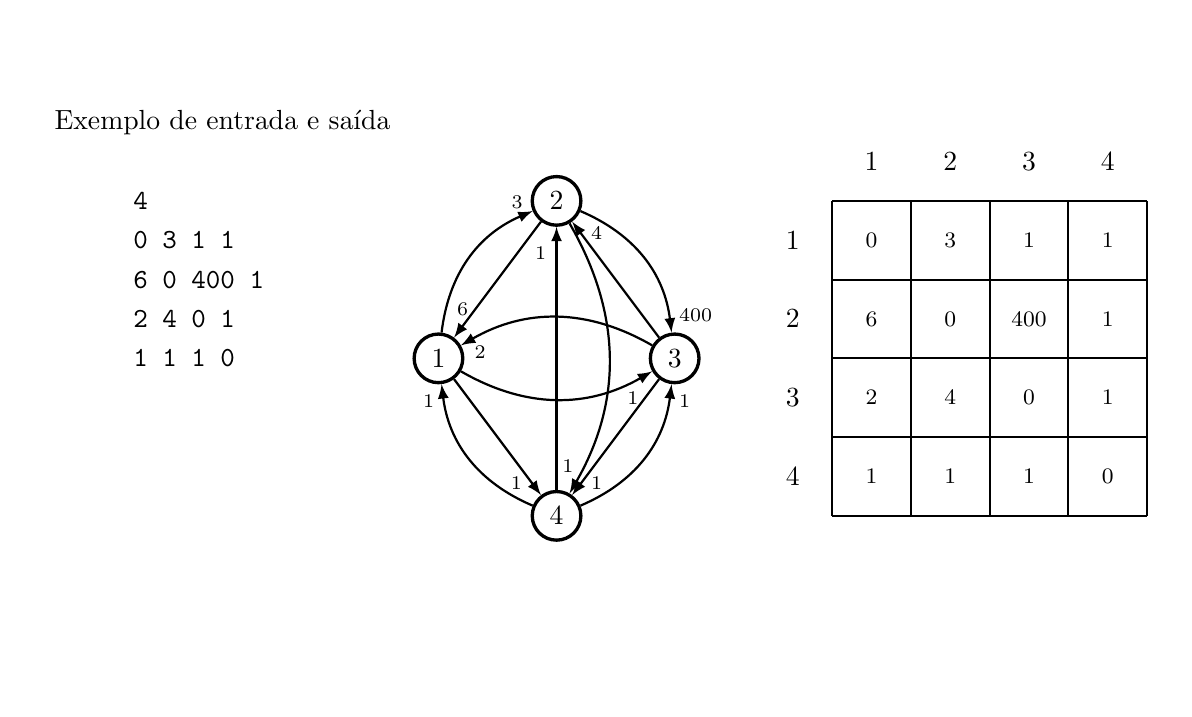
\begin{tikzpicture}
\node[draw,opacity=0] at (0, 0) {x};
\node[draw,opacity=0] at (14, 8) {x};

	\node[anchor=west] (header) at (0, 7.0) { \bbbold{Exemplo de entrada e saída} };


	\node[anchor=west] (line1) at (1.0, 6.0) { \bbtext{\texttt{4} } };


	\node[draw,very thick,circle] (node1) at (5.0, 4.0) { \bbtext{1} };

	\node[draw,very thick,circle] (node2) at (6.5, 6.0) { \bbtext{2} };

	\node[draw,very thick,circle] (node3) at (8.0, 4.0) { \bbtext{3} };

	\node[draw,very thick,circle] (node4) at (6.5, 2.0) { \bbtext{4} };


	\node[anchor=west] (line2) at (1.0, 5.5) { \bbtext{\texttt{0 3 1 1} } };

	\node[anchor=west] (line3) at (1.0, 5.0) { \bbtext{\texttt{6 0 400 1} } };

	\node[anchor=west] (line4) at (1.0, 4.5) { \bbtext{\texttt{2 4 0 1} } };

	\node[anchor=west] (line5) at (1.0, 4.0) { \bbtext{\texttt{1 1 1 0} } };


	\draw[thick] (10.0, 2.0) grid  (14.0, 6.0);

	\node[] (c1) at (9.5, 5.5) { \bbtext{1} };

	\node[] (c2) at (9.5, 4.5) { \bbtext{2} };

	\node[] (c3) at (9.5, 3.5) { \bbtext{3} };

	\node[] (c4) at (9.5, 2.5) { \bbtext{4} };

	\node[] (r1) at (10.5, 6.5) { \bbtext{1} };

	\node[] (r2) at (11.5, 6.5) { \bbtext{2} };

	\node[] (r3) at (12.5, 6.5) { \bbtext{3} };

	\node[] (r4) at (13.5, 6.5) { \bbtext{4} };

	\node[] (a11) at (10.5, 5.5) { \footnotesize $0$ };

	\node[] (a12) at (11.5, 5.5) { \footnotesize $3$ };

	\node[] (a13) at (12.5, 5.5) { \footnotesize $1$ };

	\node[] (a14) at (13.5, 5.5) { \footnotesize $1$ };

	\node[] (a21) at (10.5, 4.5) { \footnotesize $6$ };

	\node[] (a22) at (11.5, 4.5) { \footnotesize $0$ };

	\node[] (a23) at (12.5, 4.5) { \footnotesize $400$ };

	\node[] (a24) at (13.5, 4.5) { \footnotesize $1$ };

	\node[] (a31) at (10.5, 3.5) { \footnotesize $2$ };

	\node[] (a32) at (11.5, 3.5) { \footnotesize $4$ };

	\node[] (a33) at (12.5, 3.5) { \footnotesize $0$ };

	\node[] (a34) at (13.5, 3.5) { \footnotesize $1$ };

	\node[] (a41) at (10.5, 2.5) { \footnotesize $1$ };

	\node[] (a42) at (11.5, 2.5) { \footnotesize $1$ };

	\node[] (a43) at (12.5, 2.5) { \footnotesize $1$ };

	\node[] (a44) at (13.5, 2.5) { \footnotesize $0$ };

	\draw[-latex,thick](node1) to [bend left] node[above,pos=0.9] { \scriptsize \bbinfo{3} } (node2);

	\draw[-latex,thick](node1) to [bend right] node[below,pos=0.9] { \scriptsize \bbinfo{1} } (node3);

	\draw[-latex,thick](node1) to node[left,pos=0.9] { \scriptsize \bbinfo{1} } (node4);

	\draw[-latex,thick](node2) to node[above,pos=0.9] { \scriptsize \bbinfo{6} } (node1);

	\draw[-latex,thick](node2) to [bend left] node[right,pos=0.9] { \scriptsize \bbinfo{400} } (node3);

	\draw[-latex,thick](node2) to [bend left] node[left,pos=0.9] { \scriptsize \bbinfo{1} } (node4);

	\draw[-latex,thick](node3) to [bend right] node[below,pos=0.9] { \scriptsize \bbinfo{2} } (node1);

	\draw[-latex,thick](node3) to node[right,pos=0.9] { \scriptsize \bbinfo{4} } (node2);

	\draw[-latex,thick](node3) to node[right,pos=0.9] { \scriptsize \bbinfo{1} } (node4);

	\draw[-latex,thick](node4) to [bend left] node[left,pos=0.9] { \scriptsize \bbinfo{1} } (node1);

	\draw[-latex,thick](node4) to node[left,pos=0.9] { \scriptsize \bbinfo{1} } (node2);

	\draw[-latex,thick](node4) to [bend right] node[right,pos=0.9] { \scriptsize \bbinfo{1} } (node3);


\end{tikzpicture}
\end{frame}
\begin{frame}[plain,t]
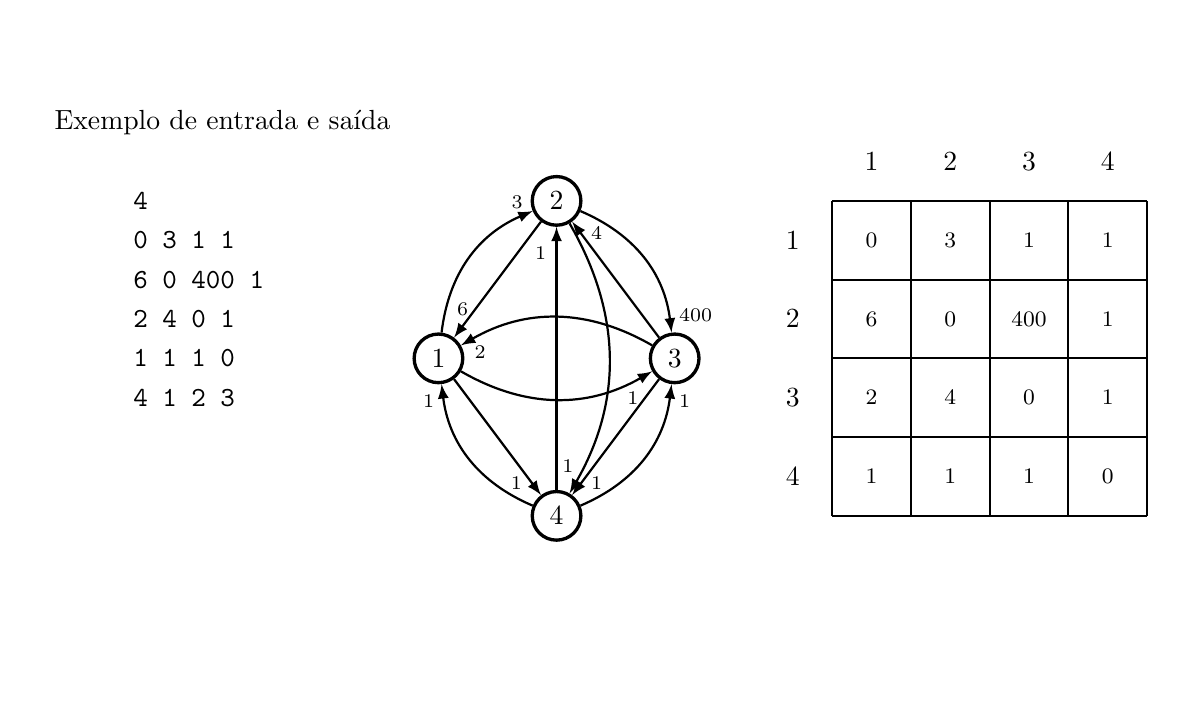
\begin{tikzpicture}
\node[draw,opacity=0] at (0, 0) {x};
\node[draw,opacity=0] at (14, 8) {x};

	\node[anchor=west] (header) at (0, 7.0) { \bbbold{Exemplo de entrada e saída} };


	\node[anchor=west] (line1) at (1.0, 6.0) { \bbtext{\texttt{4} } };


	\node[draw,very thick,circle] (node1) at (5.0, 4.0) { \bbtext{1} };

	\node[draw,very thick,circle] (node2) at (6.5, 6.0) { \bbtext{2} };

	\node[draw,very thick,circle] (node3) at (8.0, 4.0) { \bbtext{3} };

	\node[draw,very thick,circle] (node4) at (6.5, 2.0) { \bbtext{4} };


	\node[anchor=west] (line2) at (1.0, 5.5) { \bbtext{\texttt{0 3 1 1} } };

	\node[anchor=west] (line3) at (1.0, 5.0) { \bbtext{\texttt{6 0 400 1} } };

	\node[anchor=west] (line4) at (1.0, 4.5) { \bbtext{\texttt{2 4 0 1} } };

	\node[anchor=west] (line5) at (1.0, 4.0) { \bbtext{\texttt{1 1 1 0} } };


	\draw[thick] (10.0, 2.0) grid  (14.0, 6.0);

	\node[] (c1) at (9.5, 5.5) { \bbtext{1} };

	\node[] (c2) at (9.5, 4.5) { \bbtext{2} };

	\node[] (c3) at (9.5, 3.5) { \bbtext{3} };

	\node[] (c4) at (9.5, 2.5) { \bbtext{4} };

	\node[] (r1) at (10.5, 6.5) { \bbtext{1} };

	\node[] (r2) at (11.5, 6.5) { \bbtext{2} };

	\node[] (r3) at (12.5, 6.5) { \bbtext{3} };

	\node[] (r4) at (13.5, 6.5) { \bbtext{4} };

	\node[] (a11) at (10.5, 5.5) { \footnotesize $0$ };

	\node[] (a12) at (11.5, 5.5) { \footnotesize $3$ };

	\node[] (a13) at (12.5, 5.5) { \footnotesize $1$ };

	\node[] (a14) at (13.5, 5.5) { \footnotesize $1$ };

	\node[] (a21) at (10.5, 4.5) { \footnotesize $6$ };

	\node[] (a22) at (11.5, 4.5) { \footnotesize $0$ };

	\node[] (a23) at (12.5, 4.5) { \footnotesize $400$ };

	\node[] (a24) at (13.5, 4.5) { \footnotesize $1$ };

	\node[] (a31) at (10.5, 3.5) { \footnotesize $2$ };

	\node[] (a32) at (11.5, 3.5) { \footnotesize $4$ };

	\node[] (a33) at (12.5, 3.5) { \footnotesize $0$ };

	\node[] (a34) at (13.5, 3.5) { \footnotesize $1$ };

	\node[] (a41) at (10.5, 2.5) { \footnotesize $1$ };

	\node[] (a42) at (11.5, 2.5) { \footnotesize $1$ };

	\node[] (a43) at (12.5, 2.5) { \footnotesize $1$ };

	\node[] (a44) at (13.5, 2.5) { \footnotesize $0$ };

	\draw[-latex,thick](node1) to [bend left] node[above,pos=0.9] { \scriptsize \bbinfo{3} } (node2);

	\draw[-latex,thick](node1) to [bend right] node[below,pos=0.9] { \scriptsize \bbinfo{1} } (node3);

	\draw[-latex,thick](node1) to node[left,pos=0.9] { \scriptsize \bbinfo{1} } (node4);

	\draw[-latex,thick](node2) to node[above,pos=0.9] { \scriptsize \bbinfo{6} } (node1);

	\draw[-latex,thick](node2) to [bend left] node[right,pos=0.9] { \scriptsize \bbinfo{400} } (node3);

	\draw[-latex,thick](node2) to [bend left] node[left,pos=0.9] { \scriptsize \bbinfo{1} } (node4);

	\draw[-latex,thick](node3) to [bend right] node[below,pos=0.9] { \scriptsize \bbinfo{2} } (node1);

	\draw[-latex,thick](node3) to node[right,pos=0.9] { \scriptsize \bbinfo{4} } (node2);

	\draw[-latex,thick](node3) to node[right,pos=0.9] { \scriptsize \bbinfo{1} } (node4);

	\draw[-latex,thick](node4) to [bend left] node[left,pos=0.9] { \scriptsize \bbinfo{1} } (node1);

	\draw[-latex,thick](node4) to node[left,pos=0.9] { \scriptsize \bbinfo{1} } (node2);

	\draw[-latex,thick](node4) to [bend right] node[right,pos=0.9] { \scriptsize \bbinfo{1} } (node3);



	\node[anchor=west] (line6) at (1.0, 3.5) { \bbtext{\texttt{4 1 2 3} } };

\end{tikzpicture}
\end{frame}
\begin{frame}[plain,t]
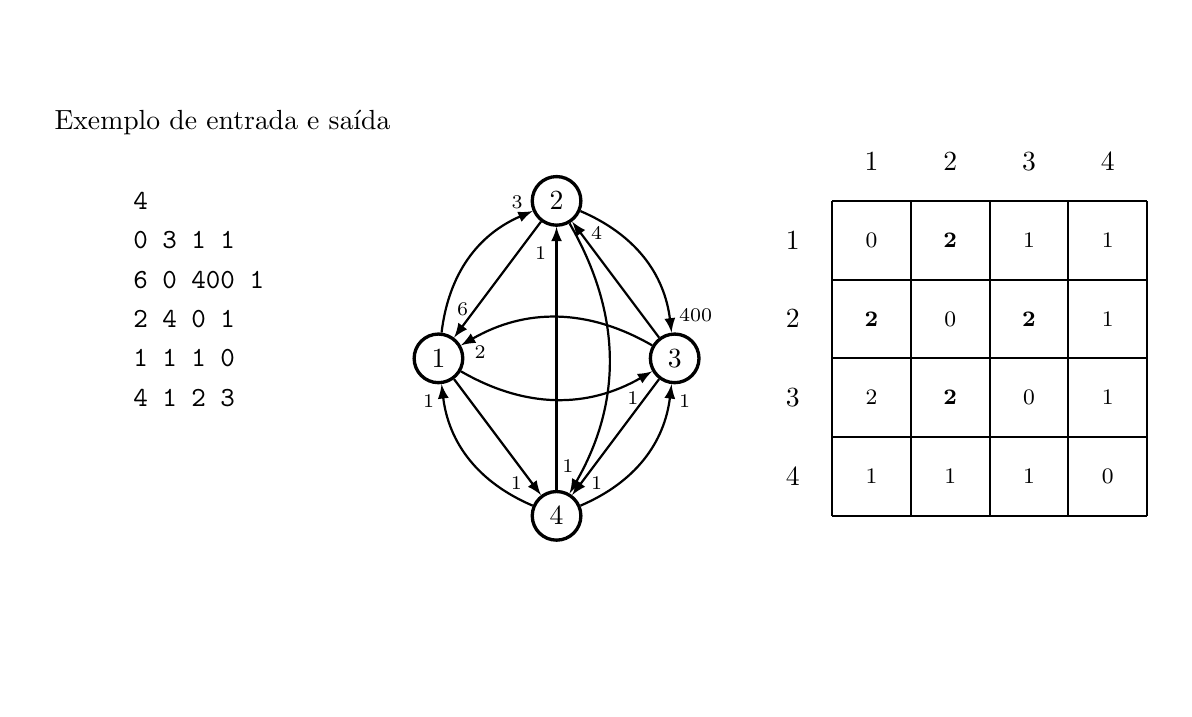
\begin{tikzpicture}
\node[draw,opacity=0] at (0, 0) {x};
\node[draw,opacity=0] at (14, 8) {x};

	\node[anchor=west] (header) at (0, 7.0) { \bbbold{Exemplo de entrada e saída} };


	\node[anchor=west] (line1) at (1.0, 6.0) { \bbtext{\texttt{4} } };


	\node[draw,very thick,circle] (node1) at (5.0, 4.0) { \bbtext{1} };

	\node[draw,very thick,circle] (node2) at (6.5, 6.0) { \bbtext{2} };

	\node[draw,very thick,circle] (node3) at (8.0, 4.0) { \bbtext{3} };

	\node[draw,very thick,circle] (node4) at (6.5, 2.0) { \bbtext{4} };


	\node[anchor=west] (line2) at (1.0, 5.5) { \bbtext{\texttt{0 3 1 1} } };

	\node[anchor=west] (line3) at (1.0, 5.0) { \bbtext{\texttt{6 0 400 1} } };

	\node[anchor=west] (line4) at (1.0, 4.5) { \bbtext{\texttt{2 4 0 1} } };

	\node[anchor=west] (line5) at (1.0, 4.0) { \bbtext{\texttt{1 1 1 0} } };


	\draw[thick] (10.0, 2.0) grid  (14.0, 6.0);

	\node[] (c1) at (9.5, 5.5) { \bbtext{1} };

	\node[] (c2) at (9.5, 4.5) { \bbtext{2} };

	\node[] (c3) at (9.5, 3.5) { \bbtext{3} };

	\node[] (c4) at (9.5, 2.5) { \bbtext{4} };

	\node[] (r1) at (10.5, 6.5) { \bbtext{1} };

	\node[] (r2) at (11.5, 6.5) { \bbtext{2} };

	\node[] (r3) at (12.5, 6.5) { \bbtext{3} };

	\node[] (r4) at (13.5, 6.5) { \bbtext{4} };

	\node[] (a11) at (10.5, 5.5) { \footnotesize $0$ };

	\node[] (a12) at (11.5, 5.5) { \footnotesize $\mathbf{2}$ };

	\node[] (a13) at (12.5, 5.5) { \footnotesize $1$ };

	\node[] (a14) at (13.5, 5.5) { \footnotesize $1$ };

	\node[] (a21) at (10.5, 4.5) { \footnotesize $\mathbf{2}$ };

	\node[] (a22) at (11.5, 4.5) { \footnotesize $0$ };

	\node[] (a23) at (12.5, 4.5) { \footnotesize $\mathbf{2}$ };

	\node[] (a24) at (13.5, 4.5) { \footnotesize $1$ };

	\node[] (a31) at (10.5, 3.5) { \footnotesize $2$ };

	\node[] (a32) at (11.5, 3.5) { \footnotesize $\mathbf{2}$ };

	\node[] (a33) at (12.5, 3.5) { \footnotesize $0$ };

	\node[] (a34) at (13.5, 3.5) { \footnotesize $1$ };

	\node[] (a41) at (10.5, 2.5) { \footnotesize $1$ };

	\node[] (a42) at (11.5, 2.5) { \footnotesize $1$ };

	\node[] (a43) at (12.5, 2.5) { \footnotesize $1$ };

	\node[] (a44) at (13.5, 2.5) { \footnotesize $0$ };

	\draw[-latex,thick](node1) to [bend left] node[above,pos=0.9] { \scriptsize \bbinfo{3} } (node2);

	\draw[-latex,thick](node1) to [bend right] node[below,pos=0.9] { \scriptsize \bbinfo{1} } (node3);

	\draw[-latex,thick](node1) to node[left,pos=0.9] { \scriptsize \bbinfo{1} } (node4);

	\draw[-latex,thick](node2) to node[above,pos=0.9] { \scriptsize \bbinfo{6} } (node1);

	\draw[-latex,thick](node2) to [bend left] node[right,pos=0.9] { \scriptsize \bbinfo{400} } (node3);

	\draw[-latex,thick](node2) to [bend left] node[left,pos=0.9] { \scriptsize \bbinfo{1} } (node4);

	\draw[-latex,thick](node3) to [bend right] node[below,pos=0.9] { \scriptsize \bbinfo{2} } (node1);

	\draw[-latex,thick](node3) to node[right,pos=0.9] { \scriptsize \bbinfo{4} } (node2);

	\draw[-latex,thick](node3) to node[right,pos=0.9] { \scriptsize \bbinfo{1} } (node4);

	\draw[-latex,thick](node4) to [bend left] node[left,pos=0.9] { \scriptsize \bbinfo{1} } (node1);

	\draw[-latex,thick](node4) to node[left,pos=0.9] { \scriptsize \bbinfo{1} } (node2);

	\draw[-latex,thick](node4) to [bend right] node[right,pos=0.9] { \scriptsize \bbinfo{1} } (node3);



	\node[anchor=west] (line6) at (1.0, 3.5) { \bbtext{\texttt{4 1 2 3} } };



\end{tikzpicture}
\end{frame}
\begin{frame}[plain,t]
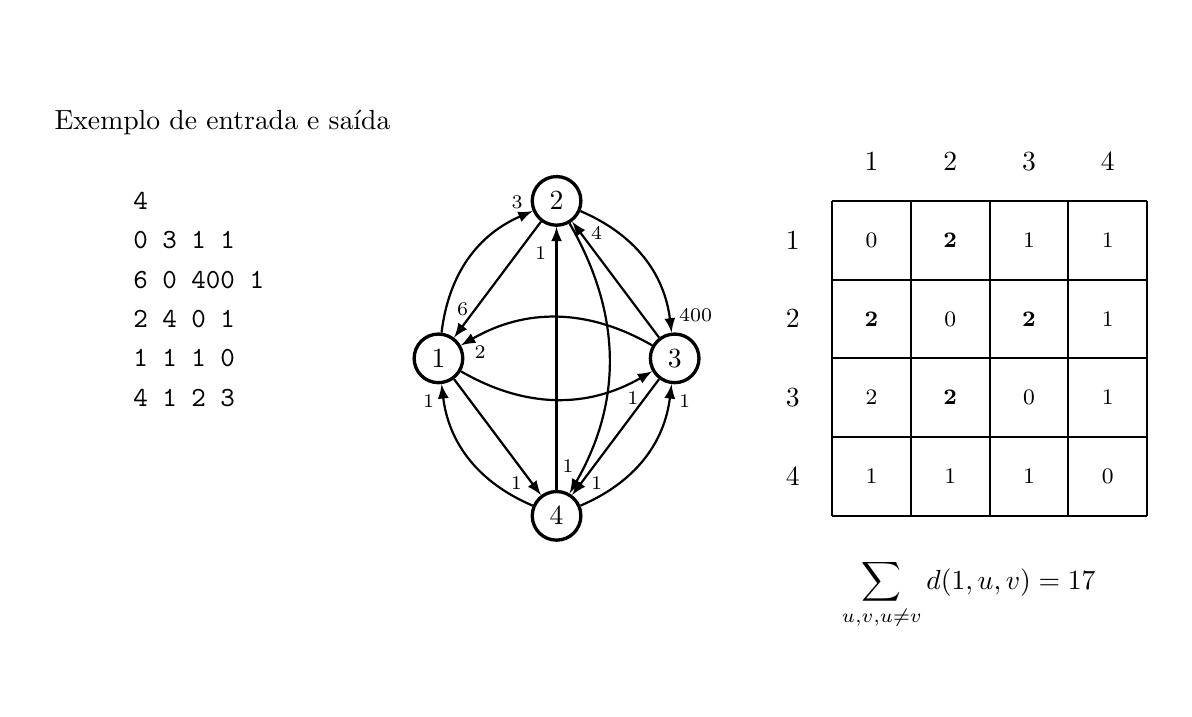
\begin{tikzpicture}
\node[draw,opacity=0] at (0, 0) {x};
\node[draw,opacity=0] at (14, 8) {x};

	\node[anchor=west] (header) at (0, 7.0) { \bbbold{Exemplo de entrada e saída} };


	\node[anchor=west] (line1) at (1.0, 6.0) { \bbtext{\texttt{4} } };


	\node[draw,very thick,circle] (node1) at (5.0, 4.0) { \bbtext{1} };

	\node[draw,very thick,circle] (node2) at (6.5, 6.0) { \bbtext{2} };

	\node[draw,very thick,circle] (node3) at (8.0, 4.0) { \bbtext{3} };

	\node[draw,very thick,circle] (node4) at (6.5, 2.0) { \bbtext{4} };


	\node[anchor=west] (line2) at (1.0, 5.5) { \bbtext{\texttt{0 3 1 1} } };

	\node[anchor=west] (line3) at (1.0, 5.0) { \bbtext{\texttt{6 0 400 1} } };

	\node[anchor=west] (line4) at (1.0, 4.5) { \bbtext{\texttt{2 4 0 1} } };

	\node[anchor=west] (line5) at (1.0, 4.0) { \bbtext{\texttt{1 1 1 0} } };


	\draw[thick] (10.0, 2.0) grid  (14.0, 6.0);

	\node[] (c1) at (9.5, 5.5) { \bbtext{1} };

	\node[] (c2) at (9.5, 4.5) { \bbtext{2} };

	\node[] (c3) at (9.5, 3.5) { \bbtext{3} };

	\node[] (c4) at (9.5, 2.5) { \bbtext{4} };

	\node[] (r1) at (10.5, 6.5) { \bbtext{1} };

	\node[] (r2) at (11.5, 6.5) { \bbtext{2} };

	\node[] (r3) at (12.5, 6.5) { \bbtext{3} };

	\node[] (r4) at (13.5, 6.5) { \bbtext{4} };

	\node[] (a11) at (10.5, 5.5) { \footnotesize $0$ };

	\node[] (a12) at (11.5, 5.5) { \footnotesize $\mathbf{2}$ };

	\node[] (a13) at (12.5, 5.5) { \footnotesize $1$ };

	\node[] (a14) at (13.5, 5.5) { \footnotesize $1$ };

	\node[] (a21) at (10.5, 4.5) { \footnotesize $\mathbf{2}$ };

	\node[] (a22) at (11.5, 4.5) { \footnotesize $0$ };

	\node[] (a23) at (12.5, 4.5) { \footnotesize $\mathbf{2}$ };

	\node[] (a24) at (13.5, 4.5) { \footnotesize $1$ };

	\node[] (a31) at (10.5, 3.5) { \footnotesize $2$ };

	\node[] (a32) at (11.5, 3.5) { \footnotesize $\mathbf{2}$ };

	\node[] (a33) at (12.5, 3.5) { \footnotesize $0$ };

	\node[] (a34) at (13.5, 3.5) { \footnotesize $1$ };

	\node[] (a41) at (10.5, 2.5) { \footnotesize $1$ };

	\node[] (a42) at (11.5, 2.5) { \footnotesize $1$ };

	\node[] (a43) at (12.5, 2.5) { \footnotesize $1$ };

	\node[] (a44) at (13.5, 2.5) { \footnotesize $0$ };

	\draw[-latex,thick](node1) to [bend left] node[above,pos=0.9] { \scriptsize \bbinfo{3} } (node2);

	\draw[-latex,thick](node1) to [bend right] node[below,pos=0.9] { \scriptsize \bbinfo{1} } (node3);

	\draw[-latex,thick](node1) to node[left,pos=0.9] { \scriptsize \bbinfo{1} } (node4);

	\draw[-latex,thick](node2) to node[above,pos=0.9] { \scriptsize \bbinfo{6} } (node1);

	\draw[-latex,thick](node2) to [bend left] node[right,pos=0.9] { \scriptsize \bbinfo{400} } (node3);

	\draw[-latex,thick](node2) to [bend left] node[left,pos=0.9] { \scriptsize \bbinfo{1} } (node4);

	\draw[-latex,thick](node3) to [bend right] node[below,pos=0.9] { \scriptsize \bbinfo{2} } (node1);

	\draw[-latex,thick](node3) to node[right,pos=0.9] { \scriptsize \bbinfo{4} } (node2);

	\draw[-latex,thick](node3) to node[right,pos=0.9] { \scriptsize \bbinfo{1} } (node4);

	\draw[-latex,thick](node4) to [bend left] node[left,pos=0.9] { \scriptsize \bbinfo{1} } (node1);

	\draw[-latex,thick](node4) to node[left,pos=0.9] { \scriptsize \bbinfo{1} } (node2);

	\draw[-latex,thick](node4) to [bend right] node[right,pos=0.9] { \scriptsize \bbinfo{1} } (node3);



	\node[anchor=west] (line6) at (1.0, 3.5) { \bbtext{\texttt{4 1 2 3} } };




	\node[anchor=west] (eq) at (10.0, 1.0) { $\displaystyle \sum_{u, v, u\neq v} d(1, u, v) = 17$ };

\end{tikzpicture}
\end{frame}
\begin{frame}[plain,t]
\begin{tikzpicture}
\node[draw,opacity=0] at (0, 0) {x};
\node[draw,opacity=0] at (14, 8) {x};

	\node[anchor=west] (header) at (0, 7.0) { \bbbold{Exemplo de entrada e saída} };


	\node[anchor=west] (line1) at (1.0, 6.0) { \bbtext{\texttt{4} } };


	\node[draw,very thick,circle] (node1) at (5.0, 4.0) { \bbtext{1} };

	\node[draw,very thick,circle] (node2) at (6.5, 6.0) { \bbtext{2} };

	\node[draw,very thick,circle] (node3) at (8.0, 4.0) { \bbtext{3} };

	\node[draw,very thick,circle,fill=BBRed] (node4) at (6.5, 2.0) { \bbtext{4} };


	\node[anchor=west] (line2) at (1.0, 5.5) { \bbtext{\texttt{0 3 1 1} } };

	\node[anchor=west] (line3) at (1.0, 5.0) { \bbtext{\texttt{6 0 400 1} } };

	\node[anchor=west] (line4) at (1.0, 4.5) { \bbtext{\texttt{2 4 0 1} } };

	\node[anchor=west] (line5) at (1.0, 4.0) { \bbtext{\texttt{1 1 1 0} } };


	\draw[thick] (10.0, 2.0) grid  (14.0, 6.0);

	\node[] (c1) at (9.5, 5.5) { \bbtext{1} };

	\node[] (c2) at (9.5, 4.5) { \bbtext{2} };

	\node[] (c3) at (9.5, 3.5) { \bbtext{3} };

	\node[] (c4) at (9.5, 2.5) { \bbtext{4} };

	\node[] (r1) at (10.5, 6.5) { \bbtext{1} };

	\node[] (r2) at (11.5, 6.5) { \bbtext{2} };

	\node[] (r3) at (12.5, 6.5) { \bbtext{3} };

	\node[] (r4) at (13.5, 6.5) { \bbtext{4} };

	\node[] (a11) at (10.5, 5.5) { \footnotesize $0$ };

	\node[] (a12) at (11.5, 5.5) { \footnotesize ${2}$ };

	\node[] (a13) at (12.5, 5.5) { \footnotesize $1$ };

	\node[] (a14) at (13.5, 5.5) { \footnotesize $1$ };

	\node[] (a21) at (10.5, 4.5) { \footnotesize ${2}$ };

	\node[] (a22) at (11.5, 4.5) { \footnotesize $0$ };

	\node[] (a23) at (12.5, 4.5) { \footnotesize ${2}$ };

	\node[] (a24) at (13.5, 4.5) { \footnotesize $1$ };

	\node[] (a31) at (10.5, 3.5) { \footnotesize $2$ };

	\node[] (a32) at (11.5, 3.5) { \footnotesize ${2}$ };

	\node[] (a33) at (12.5, 3.5) { \footnotesize $0$ };

	\node[] (a34) at (13.5, 3.5) { \footnotesize $1$ };

	\node[] (a41) at (10.5, 2.5) { \footnotesize $1$ };

	\node[] (a42) at (11.5, 2.5) { \footnotesize $1$ };

	\node[] (a43) at (12.5, 2.5) { \footnotesize $1$ };

	\node[] (a44) at (13.5, 2.5) { \footnotesize $0$ };

	\draw[-latex,thick](node1) to [bend left] node[above,pos=0.9] { \scriptsize \bbinfo{3} } (node2);

	\draw[-latex,thick](node1) to [bend right] node[below,pos=0.9] { \scriptsize \bbinfo{1} } (node3);

	\draw[-latex,thick](node1) to node[left,pos=0.9] { \scriptsize \bbinfo{1} } (node4);

	\draw[-latex,thick](node2) to node[above,pos=0.9] { \scriptsize \bbinfo{6} } (node1);

	\draw[-latex,thick](node2) to [bend left] node[right,pos=0.9] { \scriptsize \bbinfo{400} } (node3);

	\draw[-latex,thick](node2) to [bend left] node[left,pos=0.9] { \scriptsize \bbinfo{1} } (node4);

	\draw[-latex,thick](node3) to [bend right] node[below,pos=0.9] { \scriptsize \bbinfo{2} } (node1);

	\draw[-latex,thick](node3) to node[right,pos=0.9] { \scriptsize \bbinfo{4} } (node2);

	\draw[-latex,thick](node3) to node[right,pos=0.9] { \scriptsize \bbinfo{1} } (node4);

	\draw[-latex,thick](node4) to [bend left] node[left,pos=0.9] { \scriptsize \bbinfo{1} } (node1);

	\draw[-latex,thick](node4) to node[left,pos=0.9] { \scriptsize \bbinfo{1} } (node2);

	\draw[-latex,thick](node4) to [bend right] node[right,pos=0.9] { \scriptsize \bbinfo{1} } (node3);



	\node[anchor=west] (line6) at (1.0, 3.5) { \bbtext{\texttt{4 1 2 3} } };








\end{tikzpicture}
\end{frame}
\begin{frame}[plain,t]
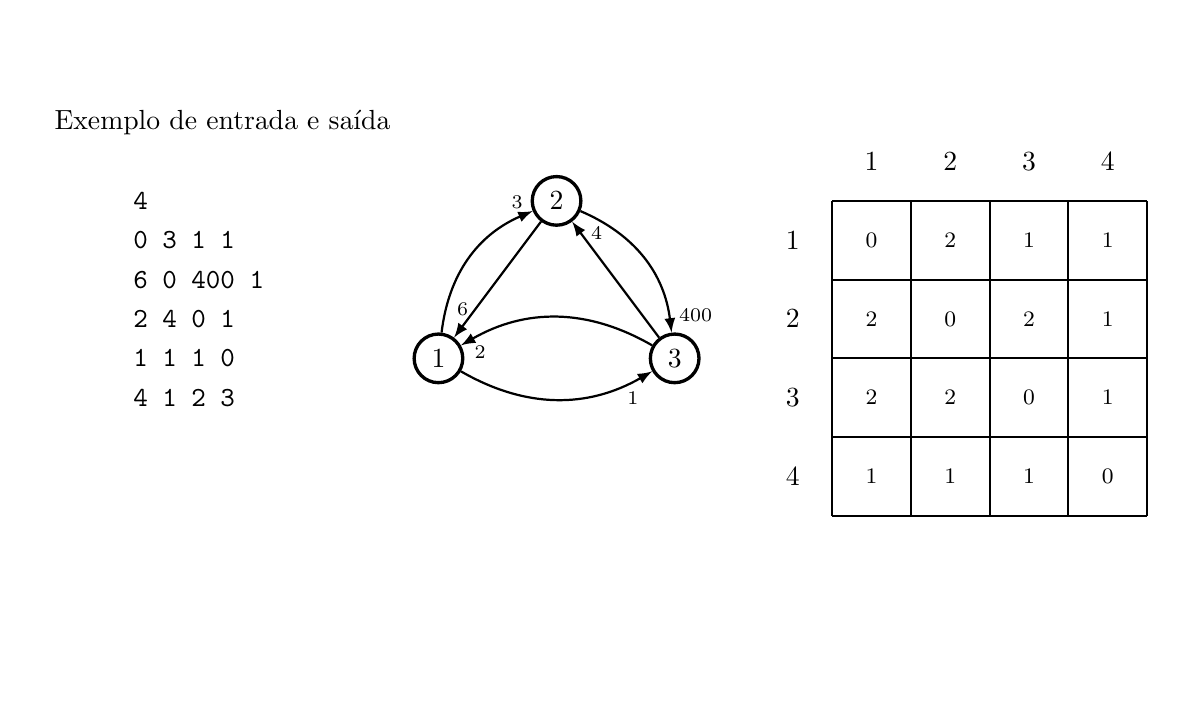
\begin{tikzpicture}
\node[draw,opacity=0] at (0, 0) {x};
\node[draw,opacity=0] at (14, 8) {x};

	\node[anchor=west] (header) at (0, 7.0) { \bbbold{Exemplo de entrada e saída} };


	\node[anchor=west] (line1) at (1.0, 6.0) { \bbtext{\texttt{4} } };


	\node[draw,very thick,circle] (node1) at (5.0, 4.0) { \bbtext{1} };

	\node[draw,very thick,circle] (node2) at (6.5, 6.0) { \bbtext{2} };

	\node[draw,very thick,circle] (node3) at (8.0, 4.0) { \bbtext{3} };



	\node[anchor=west] (line2) at (1.0, 5.5) { \bbtext{\texttt{0 3 1 1} } };

	\node[anchor=west] (line3) at (1.0, 5.0) { \bbtext{\texttt{6 0 400 1} } };

	\node[anchor=west] (line4) at (1.0, 4.5) { \bbtext{\texttt{2 4 0 1} } };

	\node[anchor=west] (line5) at (1.0, 4.0) { \bbtext{\texttt{1 1 1 0} } };


	\draw[thick] (10.0, 2.0) grid  (14.0, 6.0);

	\node[] (c1) at (9.5, 5.5) { \bbtext{1} };

	\node[] (c2) at (9.5, 4.5) { \bbtext{2} };

	\node[] (c3) at (9.5, 3.5) { \bbtext{3} };

	\node[] (c4) at (9.5, 2.5) { \bbtext{4} };

	\node[] (r1) at (10.5, 6.5) { \bbtext{1} };

	\node[] (r2) at (11.5, 6.5) { \bbtext{2} };

	\node[] (r3) at (12.5, 6.5) { \bbtext{3} };

	\node[] (r4) at (13.5, 6.5) { \bbtext{4} };

	\node[] (a11) at (10.5, 5.5) { \footnotesize $0$ };

	\node[] (a12) at (11.5, 5.5) { \footnotesize ${2}$ };

	\node[] (a13) at (12.5, 5.5) { \footnotesize $1$ };

	\node[] (a14) at (13.5, 5.5) { \footnotesize $1$ };

	\node[] (a21) at (10.5, 4.5) { \footnotesize ${2}$ };

	\node[] (a22) at (11.5, 4.5) { \footnotesize $0$ };

	\node[] (a23) at (12.5, 4.5) { \footnotesize ${2}$ };

	\node[] (a24) at (13.5, 4.5) { \footnotesize $1$ };

	\node[] (a31) at (10.5, 3.5) { \footnotesize $2$ };

	\node[] (a32) at (11.5, 3.5) { \footnotesize ${2}$ };

	\node[] (a33) at (12.5, 3.5) { \footnotesize $0$ };

	\node[] (a34) at (13.5, 3.5) { \footnotesize $1$ };

	\node[] (a41) at (10.5, 2.5) { \footnotesize $1$ };

	\node[] (a42) at (11.5, 2.5) { \footnotesize $1$ };

	\node[] (a43) at (12.5, 2.5) { \footnotesize $1$ };

	\node[] (a44) at (13.5, 2.5) { \footnotesize $0$ };

	\draw[-latex,thick](node1) to [bend left] node[above,pos=0.9] { \scriptsize \bbinfo{3} } (node2);

	\draw[-latex,thick](node1) to [bend right] node[below,pos=0.9] { \scriptsize \bbinfo{1} } (node3);


	\draw[-latex,thick](node2) to node[above,pos=0.9] { \scriptsize \bbinfo{6} } (node1);

	\draw[-latex,thick](node2) to [bend left] node[right,pos=0.9] { \scriptsize \bbinfo{400} } (node3);


	\draw[-latex,thick](node3) to [bend right] node[below,pos=0.9] { \scriptsize \bbinfo{2} } (node1);

	\draw[-latex,thick](node3) to node[right,pos=0.9] { \scriptsize \bbinfo{4} } (node2);







	\node[anchor=west] (line6) at (1.0, 3.5) { \bbtext{\texttt{4 1 2 3} } };










\end{tikzpicture}
\end{frame}
\begin{frame}[plain,t]
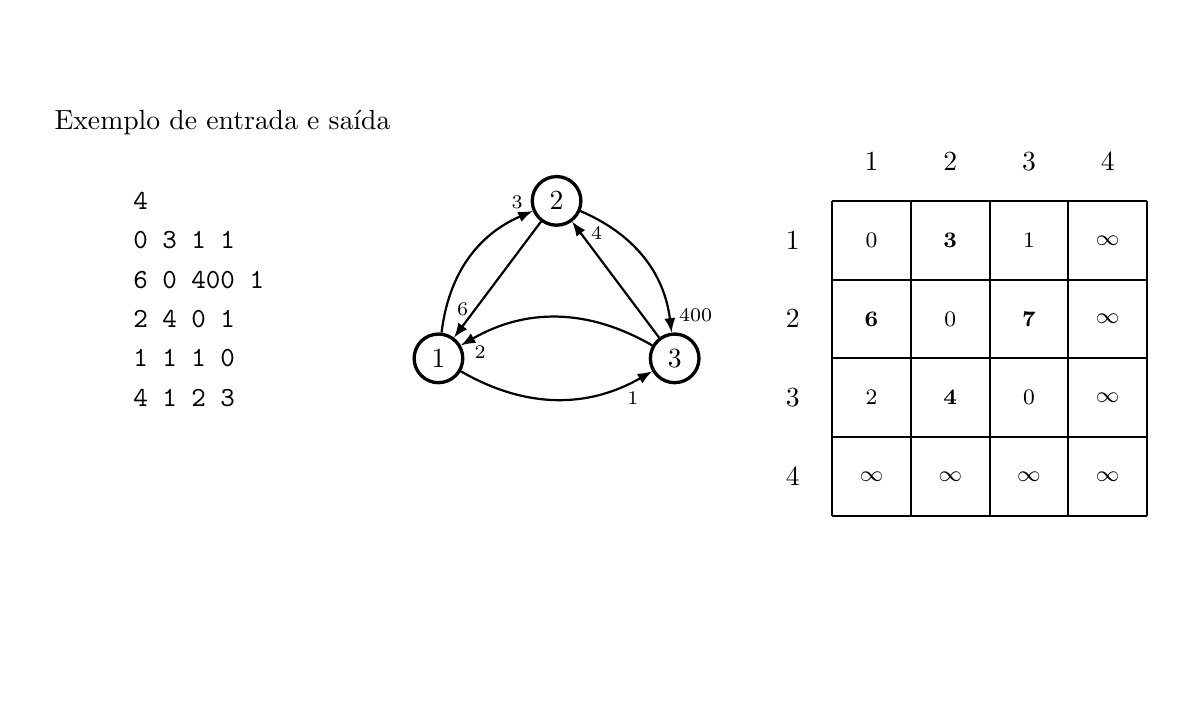
\begin{tikzpicture}
\node[draw,opacity=0] at (0, 0) {x};
\node[draw,opacity=0] at (14, 8) {x};

	\node[anchor=west] (header) at (0, 7.0) { \bbbold{Exemplo de entrada e saída} };


	\node[anchor=west] (line1) at (1.0, 6.0) { \bbtext{\texttt{4} } };


	\node[draw,very thick,circle] (node1) at (5.0, 4.0) { \bbtext{1} };

	\node[draw,very thick,circle] (node2) at (6.5, 6.0) { \bbtext{2} };

	\node[draw,very thick,circle] (node3) at (8.0, 4.0) { \bbtext{3} };



	\node[anchor=west] (line2) at (1.0, 5.5) { \bbtext{\texttt{0 3 1 1} } };

	\node[anchor=west] (line3) at (1.0, 5.0) { \bbtext{\texttt{6 0 400 1} } };

	\node[anchor=west] (line4) at (1.0, 4.5) { \bbtext{\texttt{2 4 0 1} } };

	\node[anchor=west] (line5) at (1.0, 4.0) { \bbtext{\texttt{1 1 1 0} } };


	\draw[thick] (10.0, 2.0) grid  (14.0, 6.0);

	\node[] (c1) at (9.5, 5.5) { \bbtext{1} };

	\node[] (c2) at (9.5, 4.5) { \bbtext{2} };

	\node[] (c3) at (9.5, 3.5) { \bbtext{3} };

	\node[] (c4) at (9.5, 2.5) { \bbtext{4} };

	\node[] (r1) at (10.5, 6.5) { \bbtext{1} };

	\node[] (r2) at (11.5, 6.5) { \bbtext{2} };

	\node[] (r3) at (12.5, 6.5) { \bbtext{3} };

	\node[] (r4) at (13.5, 6.5) { \bbtext{4} };

	\node[] (a11) at (10.5, 5.5) { \footnotesize $0$ };

	\node[] (a12) at (11.5, 5.5) { \footnotesize $\mathbf{3}$ };

	\node[] (a13) at (12.5, 5.5) { \footnotesize $1$ };

	\node[] (a14) at (13.5, 5.5) { \footnotesize $\infty$ };

	\node[] (a21) at (10.5, 4.5) { \footnotesize $\mathbf{6}$ };

	\node[] (a22) at (11.5, 4.5) { \footnotesize $0$ };

	\node[] (a23) at (12.5, 4.5) { \footnotesize $\mathbf{7}$ };

	\node[] (a24) at (13.5, 4.5) { \footnotesize $\infty$ };

	\node[] (a31) at (10.5, 3.5) { \footnotesize $2$ };

	\node[] (a32) at (11.5, 3.5) { \footnotesize $\mathbf{4}$ };

	\node[] (a33) at (12.5, 3.5) { \footnotesize $0$ };

	\node[] (a34) at (13.5, 3.5) { \footnotesize $\infty$ };

	\node[] (a41) at (10.5, 2.5) { \footnotesize $\infty$ };

	\node[] (a42) at (11.5, 2.5) { \footnotesize $\infty$ };

	\node[] (a43) at (12.5, 2.5) { \footnotesize $\infty$ };

	\node[] (a44) at (13.5, 2.5) { \footnotesize $\infty$ };

	\draw[-latex,thick](node1) to [bend left] node[above,pos=0.9] { \scriptsize \bbinfo{3} } (node2);

	\draw[-latex,thick](node1) to [bend right] node[below,pos=0.9] { \scriptsize \bbinfo{1} } (node3);


	\draw[-latex,thick](node2) to node[above,pos=0.9] { \scriptsize \bbinfo{6} } (node1);

	\draw[-latex,thick](node2) to [bend left] node[right,pos=0.9] { \scriptsize \bbinfo{400} } (node3);


	\draw[-latex,thick](node3) to [bend right] node[below,pos=0.9] { \scriptsize \bbinfo{2} } (node1);

	\draw[-latex,thick](node3) to node[right,pos=0.9] { \scriptsize \bbinfo{4} } (node2);







	\node[anchor=west] (line6) at (1.0, 3.5) { \bbtext{\texttt{4 1 2 3} } };












\end{tikzpicture}
\end{frame}
\begin{frame}[plain,t]
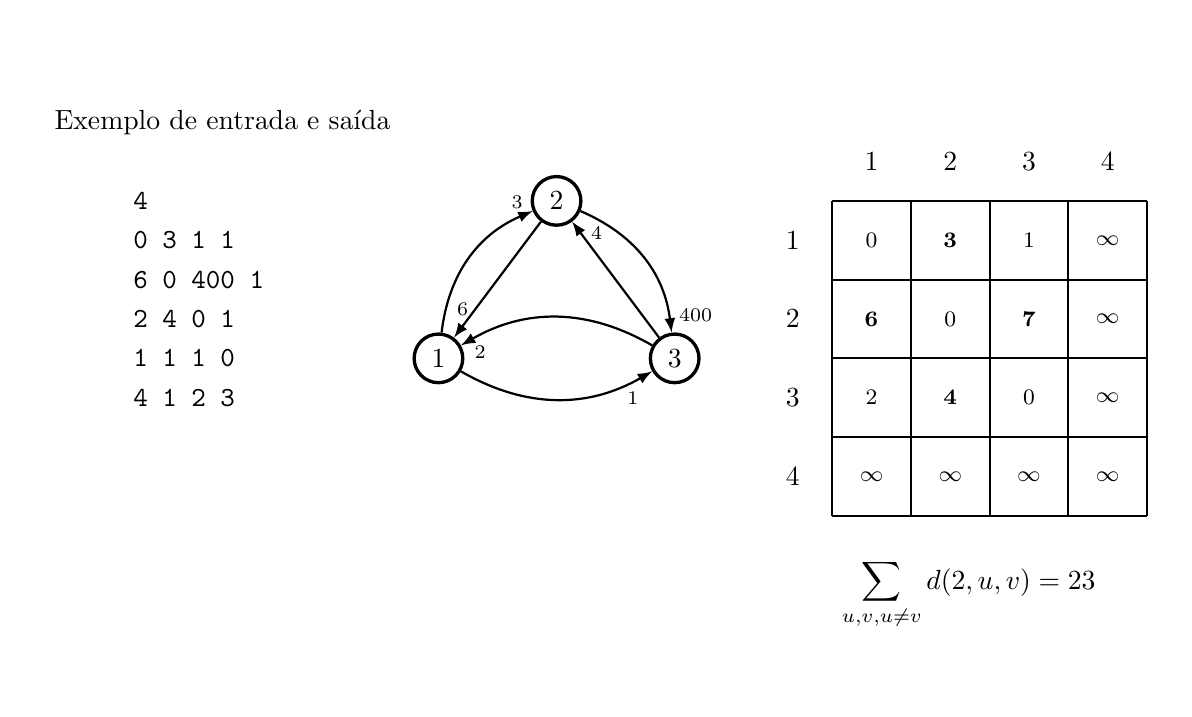
\begin{tikzpicture}
\node[draw,opacity=0] at (0, 0) {x};
\node[draw,opacity=0] at (14, 8) {x};

	\node[anchor=west] (header) at (0, 7.0) { \bbbold{Exemplo de entrada e saída} };


	\node[anchor=west] (line1) at (1.0, 6.0) { \bbtext{\texttt{4} } };


	\node[draw,very thick,circle] (node1) at (5.0, 4.0) { \bbtext{1} };

	\node[draw,very thick,circle] (node2) at (6.5, 6.0) { \bbtext{2} };

	\node[draw,very thick,circle] (node3) at (8.0, 4.0) { \bbtext{3} };



	\node[anchor=west] (line2) at (1.0, 5.5) { \bbtext{\texttt{0 3 1 1} } };

	\node[anchor=west] (line3) at (1.0, 5.0) { \bbtext{\texttt{6 0 400 1} } };

	\node[anchor=west] (line4) at (1.0, 4.5) { \bbtext{\texttt{2 4 0 1} } };

	\node[anchor=west] (line5) at (1.0, 4.0) { \bbtext{\texttt{1 1 1 0} } };


	\draw[thick] (10.0, 2.0) grid  (14.0, 6.0);

	\node[] (c1) at (9.5, 5.5) { \bbtext{1} };

	\node[] (c2) at (9.5, 4.5) { \bbtext{2} };

	\node[] (c3) at (9.5, 3.5) { \bbtext{3} };

	\node[] (c4) at (9.5, 2.5) { \bbtext{4} };

	\node[] (r1) at (10.5, 6.5) { \bbtext{1} };

	\node[] (r2) at (11.5, 6.5) { \bbtext{2} };

	\node[] (r3) at (12.5, 6.5) { \bbtext{3} };

	\node[] (r4) at (13.5, 6.5) { \bbtext{4} };

	\node[] (a11) at (10.5, 5.5) { \footnotesize $0$ };

	\node[] (a12) at (11.5, 5.5) { \footnotesize $\mathbf{3}$ };

	\node[] (a13) at (12.5, 5.5) { \footnotesize $1$ };

	\node[] (a14) at (13.5, 5.5) { \footnotesize $\infty$ };

	\node[] (a21) at (10.5, 4.5) { \footnotesize $\mathbf{6}$ };

	\node[] (a22) at (11.5, 4.5) { \footnotesize $0$ };

	\node[] (a23) at (12.5, 4.5) { \footnotesize $\mathbf{7}$ };

	\node[] (a24) at (13.5, 4.5) { \footnotesize $\infty$ };

	\node[] (a31) at (10.5, 3.5) { \footnotesize $2$ };

	\node[] (a32) at (11.5, 3.5) { \footnotesize $\mathbf{4}$ };

	\node[] (a33) at (12.5, 3.5) { \footnotesize $0$ };

	\node[] (a34) at (13.5, 3.5) { \footnotesize $\infty$ };

	\node[] (a41) at (10.5, 2.5) { \footnotesize $\infty$ };

	\node[] (a42) at (11.5, 2.5) { \footnotesize $\infty$ };

	\node[] (a43) at (12.5, 2.5) { \footnotesize $\infty$ };

	\node[] (a44) at (13.5, 2.5) { \footnotesize $\infty$ };

	\draw[-latex,thick](node1) to [bend left] node[above,pos=0.9] { \scriptsize \bbinfo{3} } (node2);

	\draw[-latex,thick](node1) to [bend right] node[below,pos=0.9] { \scriptsize \bbinfo{1} } (node3);


	\draw[-latex,thick](node2) to node[above,pos=0.9] { \scriptsize \bbinfo{6} } (node1);

	\draw[-latex,thick](node2) to [bend left] node[right,pos=0.9] { \scriptsize \bbinfo{400} } (node3);


	\draw[-latex,thick](node3) to [bend right] node[below,pos=0.9] { \scriptsize \bbinfo{2} } (node1);

	\draw[-latex,thick](node3) to node[right,pos=0.9] { \scriptsize \bbinfo{4} } (node2);







	\node[anchor=west] (line6) at (1.0, 3.5) { \bbtext{\texttt{4 1 2 3} } };




	\node[anchor=west] (eq) at (10.0, 1.0) { $\displaystyle \sum_{u, v, u\neq v} d(2, u, v) = 23$ };











\end{tikzpicture}
\end{frame}
\begin{frame}[plain,t]
\begin{tikzpicture}
\node[draw,opacity=0] at (0, 0) {x};
\node[draw,opacity=0] at (14, 8) {x};

	\node[anchor=west] (header) at (0, 7.0) { \bbbold{Exemplo de entrada e saída} };


	\node[anchor=west] (line1) at (1.0, 6.0) { \bbtext{\texttt{4} } };


	\node[draw,very thick,circle,fill=BBRed] (node1) at (5.0, 4.0) { \bbtext{1} };

	\node[draw,very thick,circle] (node2) at (6.5, 6.0) { \bbtext{2} };

	\node[draw,very thick,circle] (node3) at (8.0, 4.0) { \bbtext{3} };



	\node[anchor=west] (line2) at (1.0, 5.5) { \bbtext{\texttt{0 3 1 1} } };

	\node[anchor=west] (line3) at (1.0, 5.0) { \bbtext{\texttt{6 0 400 1} } };

	\node[anchor=west] (line4) at (1.0, 4.5) { \bbtext{\texttt{2 4 0 1} } };

	\node[anchor=west] (line5) at (1.0, 4.0) { \bbtext{\texttt{1 1 1 0} } };


	\draw[thick] (10.0, 2.0) grid  (14.0, 6.0);

	\node[] (c1) at (9.5, 5.5) { \bbtext{1} };

	\node[] (c2) at (9.5, 4.5) { \bbtext{2} };

	\node[] (c3) at (9.5, 3.5) { \bbtext{3} };

	\node[] (c4) at (9.5, 2.5) { \bbtext{4} };

	\node[] (r1) at (10.5, 6.5) { \bbtext{1} };

	\node[] (r2) at (11.5, 6.5) { \bbtext{2} };

	\node[] (r3) at (12.5, 6.5) { \bbtext{3} };

	\node[] (r4) at (13.5, 6.5) { \bbtext{4} };

	\node[] (a11) at (10.5, 5.5) { \footnotesize $0$ };

	\node[] (a12) at (11.5, 5.5) { \footnotesize ${3}$ };

	\node[] (a13) at (12.5, 5.5) { \footnotesize $1$ };

	\node[] (a14) at (13.5, 5.5) { \footnotesize $\infty$ };

	\node[] (a21) at (10.5, 4.5) { \footnotesize ${6}$ };

	\node[] (a22) at (11.5, 4.5) { \footnotesize $0$ };

	\node[] (a23) at (12.5, 4.5) { \footnotesize ${7}$ };

	\node[] (a24) at (13.5, 4.5) { \footnotesize $\infty$ };

	\node[] (a31) at (10.5, 3.5) { \footnotesize $2$ };

	\node[] (a32) at (11.5, 3.5) { \footnotesize ${4}$ };

	\node[] (a33) at (12.5, 3.5) { \footnotesize $0$ };

	\node[] (a34) at (13.5, 3.5) { \footnotesize $\infty$ };

	\node[] (a41) at (10.5, 2.5) { \footnotesize $\infty$ };

	\node[] (a42) at (11.5, 2.5) { \footnotesize $\infty$ };

	\node[] (a43) at (12.5, 2.5) { \footnotesize $\infty$ };

	\node[] (a44) at (13.5, 2.5) { \footnotesize $\infty$ };

	\draw[-latex,thick](node1) to [bend left] node[above,pos=0.9] { \scriptsize \bbinfo{3} } (node2);

	\draw[-latex,thick](node1) to [bend right] node[below,pos=0.9] { \scriptsize \bbinfo{1} } (node3);


	\draw[-latex,thick](node2) to node[above,pos=0.9] { \scriptsize \bbinfo{6} } (node1);

	\draw[-latex,thick](node2) to [bend left] node[right,pos=0.9] { \scriptsize \bbinfo{400} } (node3);


	\draw[-latex,thick](node3) to [bend right] node[below,pos=0.9] { \scriptsize \bbinfo{2} } (node1);

	\draw[-latex,thick](node3) to node[right,pos=0.9] { \scriptsize \bbinfo{4} } (node2);







	\node[anchor=west] (line6) at (1.0, 3.5) { \bbtext{\texttt{4 1 2 3} } };



















\end{tikzpicture}
\end{frame}
\begin{frame}[plain,t]
\begin{tikzpicture}
\node[draw,opacity=0] at (0, 0) {x};
\node[draw,opacity=0] at (14, 8) {x};

	\node[anchor=west] (header) at (0, 7.0) { \bbbold{Exemplo de entrada e saída} };


	\node[anchor=west] (line1) at (1.0, 6.0) { \bbtext{\texttt{4} } };



	\node[draw,very thick,circle] (node2) at (6.5, 6.0) { \bbtext{2} };

	\node[draw,very thick,circle] (node3) at (8.0, 4.0) { \bbtext{3} };



	\node[anchor=west] (line2) at (1.0, 5.5) { \bbtext{\texttt{0 3 1 1} } };

	\node[anchor=west] (line3) at (1.0, 5.0) { \bbtext{\texttt{6 0 400 1} } };

	\node[anchor=west] (line4) at (1.0, 4.5) { \bbtext{\texttt{2 4 0 1} } };

	\node[anchor=west] (line5) at (1.0, 4.0) { \bbtext{\texttt{1 1 1 0} } };


	\draw[thick] (10.0, 2.0) grid  (14.0, 6.0);

	\node[] (c1) at (9.5, 5.5) { \bbtext{1} };

	\node[] (c2) at (9.5, 4.5) { \bbtext{2} };

	\node[] (c3) at (9.5, 3.5) { \bbtext{3} };

	\node[] (c4) at (9.5, 2.5) { \bbtext{4} };

	\node[] (r1) at (10.5, 6.5) { \bbtext{1} };

	\node[] (r2) at (11.5, 6.5) { \bbtext{2} };

	\node[] (r3) at (12.5, 6.5) { \bbtext{3} };

	\node[] (r4) at (13.5, 6.5) { \bbtext{4} };

	\node[] (a11) at (10.5, 5.5) { \footnotesize $0$ };

	\node[] (a12) at (11.5, 5.5) { \footnotesize ${3}$ };

	\node[] (a13) at (12.5, 5.5) { \footnotesize $1$ };

	\node[] (a14) at (13.5, 5.5) { \footnotesize $\infty$ };

	\node[] (a21) at (10.5, 4.5) { \footnotesize ${6}$ };

	\node[] (a22) at (11.5, 4.5) { \footnotesize $0$ };

	\node[] (a23) at (12.5, 4.5) { \footnotesize ${7}$ };

	\node[] (a24) at (13.5, 4.5) { \footnotesize $\infty$ };

	\node[] (a31) at (10.5, 3.5) { \footnotesize $2$ };

	\node[] (a32) at (11.5, 3.5) { \footnotesize ${4}$ };

	\node[] (a33) at (12.5, 3.5) { \footnotesize $0$ };

	\node[] (a34) at (13.5, 3.5) { \footnotesize $\infty$ };

	\node[] (a41) at (10.5, 2.5) { \footnotesize $\infty$ };

	\node[] (a42) at (11.5, 2.5) { \footnotesize $\infty$ };

	\node[] (a43) at (12.5, 2.5) { \footnotesize $\infty$ };

	\node[] (a44) at (13.5, 2.5) { \footnotesize $\infty$ };





	\draw[-latex,thick](node2) to [bend left] node[right,pos=0.9] { \scriptsize \bbinfo{400} } (node3);



	\draw[-latex,thick](node3) to node[right,pos=0.9] { \scriptsize \bbinfo{4} } (node2);







	\node[anchor=west] (line6) at (1.0, 3.5) { \bbtext{\texttt{4 1 2 3} } };





















\end{tikzpicture}
\end{frame}
\begin{frame}[plain,t]
\begin{tikzpicture}
\node[draw,opacity=0] at (0, 0) {x};
\node[draw,opacity=0] at (14, 8) {x};

	\node[anchor=west] (header) at (0, 7.0) { \bbbold{Exemplo de entrada e saída} };


	\node[anchor=west] (line1) at (1.0, 6.0) { \bbtext{\texttt{4} } };



	\node[draw,very thick,circle] (node2) at (6.5, 6.0) { \bbtext{2} };

	\node[draw,very thick,circle] (node3) at (8.0, 4.0) { \bbtext{3} };



	\node[anchor=west] (line2) at (1.0, 5.5) { \bbtext{\texttt{0 3 1 1} } };

	\node[anchor=west] (line3) at (1.0, 5.0) { \bbtext{\texttt{6 0 400 1} } };

	\node[anchor=west] (line4) at (1.0, 4.5) { \bbtext{\texttt{2 4 0 1} } };

	\node[anchor=west] (line5) at (1.0, 4.0) { \bbtext{\texttt{1 1 1 0} } };


	\draw[thick] (10.0, 2.0) grid  (14.0, 6.0);

	\node[] (c1) at (9.5, 5.5) { \bbtext{1} };

	\node[] (c2) at (9.5, 4.5) { \bbtext{2} };

	\node[] (c3) at (9.5, 3.5) { \bbtext{3} };

	\node[] (c4) at (9.5, 2.5) { \bbtext{4} };

	\node[] (r1) at (10.5, 6.5) { \bbtext{1} };

	\node[] (r2) at (11.5, 6.5) { \bbtext{2} };

	\node[] (r3) at (12.5, 6.5) { \bbtext{3} };

	\node[] (r4) at (13.5, 6.5) { \bbtext{4} };

	\node[] (a11) at (10.5, 5.5) { \footnotesize $\infty$ };

	\node[] (a12) at (11.5, 5.5) { \footnotesize $\infty$ };

	\node[] (a13) at (12.5, 5.5) { \footnotesize $\infty$ };

	\node[] (a14) at (13.5, 5.5) { \footnotesize $\infty$ };

	\node[] (a21) at (10.5, 4.5) { \footnotesize $\infty$ };

	\node[] (a22) at (11.5, 4.5) { \footnotesize $0$ };

	\node[] (a23) at (12.5, 4.5) { \footnotesize $\mathbf{400}$ };

	\node[] (a24) at (13.5, 4.5) { \footnotesize $\infty$ };

	\node[] (a31) at (10.5, 3.5) { \footnotesize $\infty$ };

	\node[] (a32) at (11.5, 3.5) { \footnotesize ${4}$ };

	\node[] (a33) at (12.5, 3.5) { \footnotesize $0$ };

	\node[] (a34) at (13.5, 3.5) { \footnotesize $\infty$ };

	\node[] (a41) at (10.5, 2.5) { \footnotesize $\infty$ };

	\node[] (a42) at (11.5, 2.5) { \footnotesize $\infty$ };

	\node[] (a43) at (12.5, 2.5) { \footnotesize $\infty$ };

	\node[] (a44) at (13.5, 2.5) { \footnotesize $\infty$ };





	\draw[-latex,thick](node2) to [bend left] node[right,pos=0.9] { \scriptsize \bbinfo{400} } (node3);



	\draw[-latex,thick](node3) to node[right,pos=0.9] { \scriptsize \bbinfo{4} } (node2);







	\node[anchor=west] (line6) at (1.0, 3.5) { \bbtext{\texttt{4 1 2 3} } };






















\end{tikzpicture}
\end{frame}
\begin{frame}[plain,t]
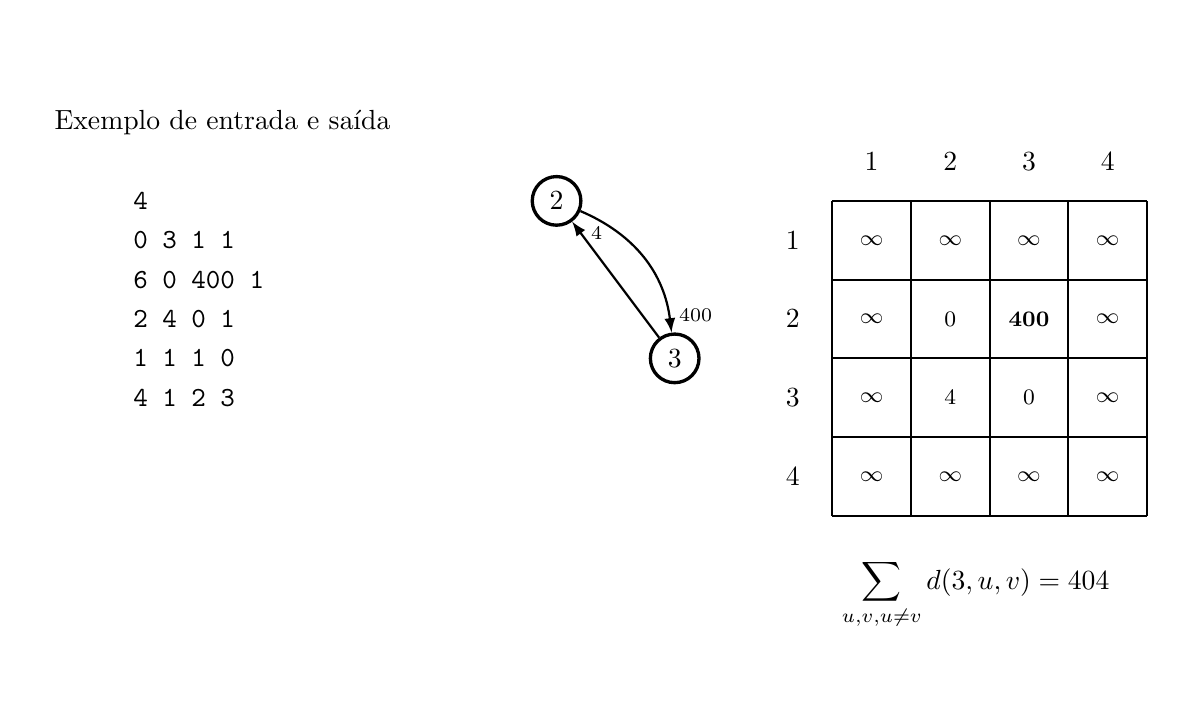
\begin{tikzpicture}
\node[draw,opacity=0] at (0, 0) {x};
\node[draw,opacity=0] at (14, 8) {x};

	\node[anchor=west] (header) at (0, 7.0) { \bbbold{Exemplo de entrada e saída} };


	\node[anchor=west] (line1) at (1.0, 6.0) { \bbtext{\texttt{4} } };



	\node[draw,very thick,circle] (node2) at (6.5, 6.0) { \bbtext{2} };

	\node[draw,very thick,circle] (node3) at (8.0, 4.0) { \bbtext{3} };



	\node[anchor=west] (line2) at (1.0, 5.5) { \bbtext{\texttt{0 3 1 1} } };

	\node[anchor=west] (line3) at (1.0, 5.0) { \bbtext{\texttt{6 0 400 1} } };

	\node[anchor=west] (line4) at (1.0, 4.5) { \bbtext{\texttt{2 4 0 1} } };

	\node[anchor=west] (line5) at (1.0, 4.0) { \bbtext{\texttt{1 1 1 0} } };


	\draw[thick] (10.0, 2.0) grid  (14.0, 6.0);

	\node[] (c1) at (9.5, 5.5) { \bbtext{1} };

	\node[] (c2) at (9.5, 4.5) { \bbtext{2} };

	\node[] (c3) at (9.5, 3.5) { \bbtext{3} };

	\node[] (c4) at (9.5, 2.5) { \bbtext{4} };

	\node[] (r1) at (10.5, 6.5) { \bbtext{1} };

	\node[] (r2) at (11.5, 6.5) { \bbtext{2} };

	\node[] (r3) at (12.5, 6.5) { \bbtext{3} };

	\node[] (r4) at (13.5, 6.5) { \bbtext{4} };

	\node[] (a11) at (10.5, 5.5) { \footnotesize $\infty$ };

	\node[] (a12) at (11.5, 5.5) { \footnotesize $\infty$ };

	\node[] (a13) at (12.5, 5.5) { \footnotesize $\infty$ };

	\node[] (a14) at (13.5, 5.5) { \footnotesize $\infty$ };

	\node[] (a21) at (10.5, 4.5) { \footnotesize $\infty$ };

	\node[] (a22) at (11.5, 4.5) { \footnotesize $0$ };

	\node[] (a23) at (12.5, 4.5) { \footnotesize $\mathbf{400}$ };

	\node[] (a24) at (13.5, 4.5) { \footnotesize $\infty$ };

	\node[] (a31) at (10.5, 3.5) { \footnotesize $\infty$ };

	\node[] (a32) at (11.5, 3.5) { \footnotesize ${4}$ };

	\node[] (a33) at (12.5, 3.5) { \footnotesize $0$ };

	\node[] (a34) at (13.5, 3.5) { \footnotesize $\infty$ };

	\node[] (a41) at (10.5, 2.5) { \footnotesize $\infty$ };

	\node[] (a42) at (11.5, 2.5) { \footnotesize $\infty$ };

	\node[] (a43) at (12.5, 2.5) { \footnotesize $\infty$ };

	\node[] (a44) at (13.5, 2.5) { \footnotesize $\infty$ };





	\draw[-latex,thick](node2) to [bend left] node[right,pos=0.9] { \scriptsize \bbinfo{400} } (node3);



	\draw[-latex,thick](node3) to node[right,pos=0.9] { \scriptsize \bbinfo{4} } (node2);







	\node[anchor=west] (line6) at (1.0, 3.5) { \bbtext{\texttt{4 1 2 3} } };




	\node[anchor=west] (eq) at (10.0, 1.0) { $\displaystyle \sum_{u, v, u\neq v} d(3, u, v) = 404$ };





















\end{tikzpicture}
\end{frame}
\begin{frame}[plain,t]
\begin{tikzpicture}
\node[draw,opacity=0] at (0, 0) {x};
\node[draw,opacity=0] at (14, 8) {x};

	\node[anchor=west] (header) at (0, 7.0) { \bbbold{Exemplo de entrada e saída} };


	\node[anchor=west] (line1) at (1.0, 6.0) { \bbtext{\texttt{4} } };



	\node[draw,very thick,circle,fill=BBRed] (node2) at (6.5, 6.0) { \bbtext{2} };

	\node[draw,very thick,circle] (node3) at (8.0, 4.0) { \bbtext{3} };



	\node[anchor=west] (line2) at (1.0, 5.5) { \bbtext{\texttt{0 3 1 1} } };

	\node[anchor=west] (line3) at (1.0, 5.0) { \bbtext{\texttt{6 0 400 1} } };

	\node[anchor=west] (line4) at (1.0, 4.5) { \bbtext{\texttt{2 4 0 1} } };

	\node[anchor=west] (line5) at (1.0, 4.0) { \bbtext{\texttt{1 1 1 0} } };


	\draw[thick] (10.0, 2.0) grid  (14.0, 6.0);

	\node[] (c1) at (9.5, 5.5) { \bbtext{1} };

	\node[] (c2) at (9.5, 4.5) { \bbtext{2} };

	\node[] (c3) at (9.5, 3.5) { \bbtext{3} };

	\node[] (c4) at (9.5, 2.5) { \bbtext{4} };

	\node[] (r1) at (10.5, 6.5) { \bbtext{1} };

	\node[] (r2) at (11.5, 6.5) { \bbtext{2} };

	\node[] (r3) at (12.5, 6.5) { \bbtext{3} };

	\node[] (r4) at (13.5, 6.5) { \bbtext{4} };

	\node[] (a11) at (10.5, 5.5) { \footnotesize $\infty$ };

	\node[] (a12) at (11.5, 5.5) { \footnotesize $\infty$ };

	\node[] (a13) at (12.5, 5.5) { \footnotesize $\infty$ };

	\node[] (a14) at (13.5, 5.5) { \footnotesize $\infty$ };

	\node[] (a21) at (10.5, 4.5) { \footnotesize $\infty$ };

	\node[] (a22) at (11.5, 4.5) { \footnotesize $0$ };

	\node[] (a23) at (12.5, 4.5) { \footnotesize ${400}$ };

	\node[] (a24) at (13.5, 4.5) { \footnotesize $\infty$ };

	\node[] (a31) at (10.5, 3.5) { \footnotesize $\infty$ };

	\node[] (a32) at (11.5, 3.5) { \footnotesize ${4}$ };

	\node[] (a33) at (12.5, 3.5) { \footnotesize $0$ };

	\node[] (a34) at (13.5, 3.5) { \footnotesize $\infty$ };

	\node[] (a41) at (10.5, 2.5) { \footnotesize $\infty$ };

	\node[] (a42) at (11.5, 2.5) { \footnotesize $\infty$ };

	\node[] (a43) at (12.5, 2.5) { \footnotesize $\infty$ };

	\node[] (a44) at (13.5, 2.5) { \footnotesize $\infty$ };





	\draw[-latex,thick](node2) to [bend left] node[right,pos=0.9] { \scriptsize \bbinfo{400} } (node3);



	\draw[-latex,thick](node3) to node[right,pos=0.9] { \scriptsize \bbinfo{4} } (node2);







	\node[anchor=west] (line6) at (1.0, 3.5) { \bbtext{\texttt{4 1 2 3} } };





























\end{tikzpicture}
\end{frame}
\begin{frame}[plain,t]
\begin{tikzpicture}
\node[draw,opacity=0] at (0, 0) {x};
\node[draw,opacity=0] at (14, 8) {x};

	\node[anchor=west] (header) at (0, 7.0) { \bbbold{Exemplo de entrada e saída} };


	\node[anchor=west] (line1) at (1.0, 6.0) { \bbtext{\texttt{4} } };




	\node[draw,very thick,circle] (node3) at (8.0, 4.0) { \bbtext{3} };



	\node[anchor=west] (line2) at (1.0, 5.5) { \bbtext{\texttt{0 3 1 1} } };

	\node[anchor=west] (line3) at (1.0, 5.0) { \bbtext{\texttt{6 0 400 1} } };

	\node[anchor=west] (line4) at (1.0, 4.5) { \bbtext{\texttt{2 4 0 1} } };

	\node[anchor=west] (line5) at (1.0, 4.0) { \bbtext{\texttt{1 1 1 0} } };


	\draw[thick] (10.0, 2.0) grid  (14.0, 6.0);

	\node[] (c1) at (9.5, 5.5) { \bbtext{1} };

	\node[] (c2) at (9.5, 4.5) { \bbtext{2} };

	\node[] (c3) at (9.5, 3.5) { \bbtext{3} };

	\node[] (c4) at (9.5, 2.5) { \bbtext{4} };

	\node[] (r1) at (10.5, 6.5) { \bbtext{1} };

	\node[] (r2) at (11.5, 6.5) { \bbtext{2} };

	\node[] (r3) at (12.5, 6.5) { \bbtext{3} };

	\node[] (r4) at (13.5, 6.5) { \bbtext{4} };

	\node[] (a11) at (10.5, 5.5) { \footnotesize $\infty$ };

	\node[] (a12) at (11.5, 5.5) { \footnotesize $\infty$ };

	\node[] (a13) at (12.5, 5.5) { \footnotesize $\infty$ };

	\node[] (a14) at (13.5, 5.5) { \footnotesize $\infty$ };

	\node[] (a21) at (10.5, 4.5) { \footnotesize $\infty$ };

	\node[] (a22) at (11.5, 4.5) { \footnotesize $0$ };

	\node[] (a23) at (12.5, 4.5) { \footnotesize ${400}$ };

	\node[] (a24) at (13.5, 4.5) { \footnotesize $\infty$ };

	\node[] (a31) at (10.5, 3.5) { \footnotesize $\infty$ };

	\node[] (a32) at (11.5, 3.5) { \footnotesize ${4}$ };

	\node[] (a33) at (12.5, 3.5) { \footnotesize $0$ };

	\node[] (a34) at (13.5, 3.5) { \footnotesize $\infty$ };

	\node[] (a41) at (10.5, 2.5) { \footnotesize $\infty$ };

	\node[] (a42) at (11.5, 2.5) { \footnotesize $\infty$ };

	\node[] (a43) at (12.5, 2.5) { \footnotesize $\infty$ };

	\node[] (a44) at (13.5, 2.5) { \footnotesize $\infty$ };















	\node[anchor=west] (line6) at (1.0, 3.5) { \bbtext{\texttt{4 1 2 3} } };































\end{tikzpicture}
\end{frame}
\begin{frame}[plain,t]
\begin{tikzpicture}
\node[draw,opacity=0] at (0, 0) {x};
\node[draw,opacity=0] at (14, 8) {x};

	\node[anchor=west] (header) at (0, 7.0) { \bbbold{Exemplo de entrada e saída} };


	\node[anchor=west] (line1) at (1.0, 6.0) { \bbtext{\texttt{4} } };




	\node[draw,very thick,circle] (node3) at (8.0, 4.0) { \bbtext{3} };



	\node[anchor=west] (line2) at (1.0, 5.5) { \bbtext{\texttt{0 3 1 1} } };

	\node[anchor=west] (line3) at (1.0, 5.0) { \bbtext{\texttt{6 0 400 1} } };

	\node[anchor=west] (line4) at (1.0, 4.5) { \bbtext{\texttt{2 4 0 1} } };

	\node[anchor=west] (line5) at (1.0, 4.0) { \bbtext{\texttt{1 1 1 0} } };


	\draw[thick] (10.0, 2.0) grid  (14.0, 6.0);

	\node[] (c1) at (9.5, 5.5) { \bbtext{1} };

	\node[] (c2) at (9.5, 4.5) { \bbtext{2} };

	\node[] (c3) at (9.5, 3.5) { \bbtext{3} };

	\node[] (c4) at (9.5, 2.5) { \bbtext{4} };

	\node[] (r1) at (10.5, 6.5) { \bbtext{1} };

	\node[] (r2) at (11.5, 6.5) { \bbtext{2} };

	\node[] (r3) at (12.5, 6.5) { \bbtext{3} };

	\node[] (r4) at (13.5, 6.5) { \bbtext{4} };

	\node[] (a11) at (10.5, 5.5) { \footnotesize $\infty$ };

	\node[] (a12) at (11.5, 5.5) { \footnotesize $\infty$ };

	\node[] (a13) at (12.5, 5.5) { \footnotesize $\infty$ };

	\node[] (a14) at (13.5, 5.5) { \footnotesize $\infty$ };

	\node[] (a21) at (10.5, 4.5) { \footnotesize $\infty$ };

	\node[] (a22) at (11.5, 4.5) { \footnotesize $\infty$ };

	\node[] (a23) at (12.5, 4.5) { \footnotesize $\infty$ };

	\node[] (a24) at (13.5, 4.5) { \footnotesize $\infty$ };

	\node[] (a31) at (10.5, 3.5) { \footnotesize $\infty$ };

	\node[] (a32) at (11.5, 3.5) { \footnotesize $\infty$ };

	\node[] (a33) at (12.5, 3.5) { \footnotesize $0$ };

	\node[] (a34) at (13.5, 3.5) { \footnotesize $\infty$ };

	\node[] (a41) at (10.5, 2.5) { \footnotesize $\infty$ };

	\node[] (a42) at (11.5, 2.5) { \footnotesize $\infty$ };

	\node[] (a43) at (12.5, 2.5) { \footnotesize $\infty$ };

	\node[] (a44) at (13.5, 2.5) { \footnotesize $\infty$ };















	\node[anchor=west] (line6) at (1.0, 3.5) { \bbtext{\texttt{4 1 2 3} } };

































\end{tikzpicture}
\end{frame}
\begin{frame}[plain,t]
\begin{tikzpicture}
\node[draw,opacity=0] at (0, 0) {x};
\node[draw,opacity=0] at (14, 8) {x};

	\node[anchor=west] (header) at (0, 7.0) { \bbbold{Exemplo de entrada e saída} };


	\node[anchor=west] (line1) at (1.0, 6.0) { \bbtext{\texttt{4} } };




	\node[draw,very thick,circle] (node3) at (8.0, 4.0) { \bbtext{3} };



	\node[anchor=west] (line2) at (1.0, 5.5) { \bbtext{\texttt{0 3 1 1} } };

	\node[anchor=west] (line3) at (1.0, 5.0) { \bbtext{\texttt{6 0 400 1} } };

	\node[anchor=west] (line4) at (1.0, 4.5) { \bbtext{\texttt{2 4 0 1} } };

	\node[anchor=west] (line5) at (1.0, 4.0) { \bbtext{\texttt{1 1 1 0} } };


	\draw[thick] (10.0, 2.0) grid  (14.0, 6.0);

	\node[] (c1) at (9.5, 5.5) { \bbtext{1} };

	\node[] (c2) at (9.5, 4.5) { \bbtext{2} };

	\node[] (c3) at (9.5, 3.5) { \bbtext{3} };

	\node[] (c4) at (9.5, 2.5) { \bbtext{4} };

	\node[] (r1) at (10.5, 6.5) { \bbtext{1} };

	\node[] (r2) at (11.5, 6.5) { \bbtext{2} };

	\node[] (r3) at (12.5, 6.5) { \bbtext{3} };

	\node[] (r4) at (13.5, 6.5) { \bbtext{4} };

	\node[] (a11) at (10.5, 5.5) { \footnotesize $\infty$ };

	\node[] (a12) at (11.5, 5.5) { \footnotesize $\infty$ };

	\node[] (a13) at (12.5, 5.5) { \footnotesize $\infty$ };

	\node[] (a14) at (13.5, 5.5) { \footnotesize $\infty$ };

	\node[] (a21) at (10.5, 4.5) { \footnotesize $\infty$ };

	\node[] (a22) at (11.5, 4.5) { \footnotesize $\infty$ };

	\node[] (a23) at (12.5, 4.5) { \footnotesize $\infty$ };

	\node[] (a24) at (13.5, 4.5) { \footnotesize $\infty$ };

	\node[] (a31) at (10.5, 3.5) { \footnotesize $\infty$ };

	\node[] (a32) at (11.5, 3.5) { \footnotesize $\infty$ };

	\node[] (a33) at (12.5, 3.5) { \footnotesize $0$ };

	\node[] (a34) at (13.5, 3.5) { \footnotesize $\infty$ };

	\node[] (a41) at (10.5, 2.5) { \footnotesize $\infty$ };

	\node[] (a42) at (11.5, 2.5) { \footnotesize $\infty$ };

	\node[] (a43) at (12.5, 2.5) { \footnotesize $\infty$ };

	\node[] (a44) at (13.5, 2.5) { \footnotesize $\infty$ };















	\node[anchor=west] (line6) at (1.0, 3.5) { \bbtext{\texttt{4 1 2 3} } };




	\node[anchor=west] (eq) at (10.0, 1.0) { $\displaystyle \sum_{u, v, u\neq v} d(4, u, v) = 0$ };
































\end{tikzpicture}
\end{frame}
\begin{frame}[plain,t]
\begin{tikzpicture}
\node[draw,opacity=0] at (0, 0) {x};
\node[draw,opacity=0] at (14, 8) {x};

	\node[anchor=west] (header) at (0, 7.0) { \bbbold{Exemplo de entrada e saída} };


	\node[anchor=west] (line1) at (1.0, 6.0) { \bbtext{\texttt{4} } };




	\node[draw,very thick,circle] (node3) at (8.0, 4.0) { \bbtext{3} };



	\node[anchor=west] (line2) at (1.0, 5.5) { \bbtext{\texttt{0 3 1 1} } };

	\node[anchor=west] (line3) at (1.0, 5.0) { \bbtext{\texttt{6 0 400 1} } };

	\node[anchor=west] (line4) at (1.0, 4.5) { \bbtext{\texttt{2 4 0 1} } };

	\node[anchor=west] (line5) at (1.0, 4.0) { \bbtext{\texttt{1 1 1 0} } };


	\draw[thick] (10.0, 2.0) grid  (14.0, 6.0);

	\node[] (c1) at (9.5, 5.5) { \bbtext{1} };

	\node[] (c2) at (9.5, 4.5) { \bbtext{2} };

	\node[] (c3) at (9.5, 3.5) { \bbtext{3} };

	\node[] (c4) at (9.5, 2.5) { \bbtext{4} };

	\node[] (r1) at (10.5, 6.5) { \bbtext{1} };

	\node[] (r2) at (11.5, 6.5) { \bbtext{2} };

	\node[] (r3) at (12.5, 6.5) { \bbtext{3} };

	\node[] (r4) at (13.5, 6.5) { \bbtext{4} };

	\node[] (a11) at (10.5, 5.5) { \footnotesize $\infty$ };

	\node[] (a12) at (11.5, 5.5) { \footnotesize $\infty$ };

	\node[] (a13) at (12.5, 5.5) { \footnotesize $\infty$ };

	\node[] (a14) at (13.5, 5.5) { \footnotesize $\infty$ };

	\node[] (a21) at (10.5, 4.5) { \footnotesize $\infty$ };

	\node[] (a22) at (11.5, 4.5) { \footnotesize $\infty$ };

	\node[] (a23) at (12.5, 4.5) { \footnotesize $\infty$ };

	\node[] (a24) at (13.5, 4.5) { \footnotesize $\infty$ };

	\node[] (a31) at (10.5, 3.5) { \footnotesize $\infty$ };

	\node[] (a32) at (11.5, 3.5) { \footnotesize $\infty$ };

	\node[] (a33) at (12.5, 3.5) { \footnotesize $0$ };

	\node[] (a34) at (13.5, 3.5) { \footnotesize $\infty$ };

	\node[] (a41) at (10.5, 2.5) { \footnotesize $\infty$ };

	\node[] (a42) at (11.5, 2.5) { \footnotesize $\infty$ };

	\node[] (a43) at (12.5, 2.5) { \footnotesize $\infty$ };

	\node[] (a44) at (13.5, 2.5) { \footnotesize $\infty$ };















	\node[anchor=west] (line6) at (1.0, 3.5) { \bbtext{\texttt{4 1 2 3} } };




	\node[anchor=west] (eq) at (10.0, 1.0) { $\displaystyle \sum_{u, v, u\neq v} d(4, u, v) = 0$ };

































	\draw[-latex,very thick,color=BBBlack] (1.85, 3.25) to  (1.85, 2.25);

	\node[] (r) at (1.85, 2.0) { \bbinfo{17 23 404 0} };

\end{tikzpicture}
\end{frame}
\begin{frame}[plain,t]
\begin{tikzpicture}
\node[draw,opacity=0] at (0, 0) {x};
\node[draw,opacity=0] at (14, 8) {x};

	\node[anchor=west] (header) at (0.0, 7.0) { \Large \bbbold{Solução} };

\end{tikzpicture}
\end{frame}
\begin{frame}[plain,t]
\begin{tikzpicture}
\node[draw,opacity=0] at (0, 0) {x};
\node[draw,opacity=0] at (14, 8) {x};

	\node[anchor=west] (header) at (0.0, 7.0) { \Large \bbbold{Solução} };


	\node[anchor=west] (line1) at (1.0, 6.0) { $\star$ \bbtext{As arestas de um vértice podem ser removidas da matriz de adjacências} };

	\node[anchor=west] (line1a) at (0.5, 5.5) { \bbtext{em $O(N)$} };

\end{tikzpicture}
\end{frame}
\begin{frame}[plain,t]
\begin{tikzpicture}
\node[draw,opacity=0] at (0, 0) {x};
\node[draw,opacity=0] at (14, 8) {x};

	\node[anchor=west] (header) at (0.0, 7.0) { \Large \bbbold{Solução} };


	\node[anchor=west] (line1) at (1.0, 6.0) { $\star$ \bbtext{As arestas de um vértice podem ser removidas da matriz de adjacências} };

	\node[anchor=west] (line1a) at (0.5, 5.5) { \bbtext{em $O(N)$} };


	\node[anchor=west] (line2) at (1.0, 4.5) { $\star$ \bbtext{Em cada etapa, os caminhos mínimos entre todos os pares podem ser} };

	\node[anchor=west] (line2a) at (0.5, 4.0) { \bbtext{computados com Floyd-Warshall em $O(N^3)$} };

\end{tikzpicture}
\end{frame}
\begin{frame}[plain,t]
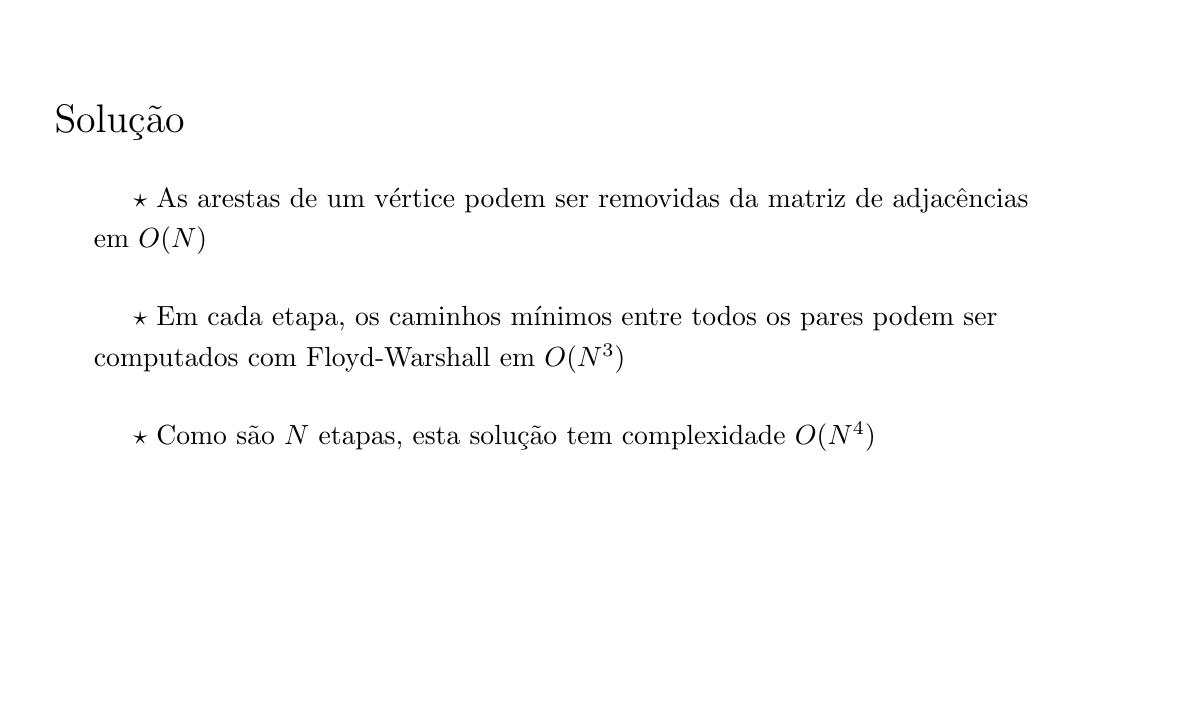
\begin{tikzpicture}
\node[draw,opacity=0] at (0, 0) {x};
\node[draw,opacity=0] at (14, 8) {x};

	\node[anchor=west] (header) at (0.0, 7.0) { \Large \bbbold{Solução} };


	\node[anchor=west] (line1) at (1.0, 6.0) { $\star$ \bbtext{As arestas de um vértice podem ser removidas da matriz de adjacências} };

	\node[anchor=west] (line1a) at (0.5, 5.5) { \bbtext{em $O(N)$} };


	\node[anchor=west] (line2) at (1.0, 4.5) { $\star$ \bbtext{Em cada etapa, os caminhos mínimos entre todos os pares podem ser} };

	\node[anchor=west] (line2a) at (0.5, 4.0) { \bbtext{computados com Floyd-Warshall em $O(N^3)$} };


	\node[anchor=west] (line3) at (1.0, 3.0) { $\star$ \bbtext{Como são $N$ etapas, esta solução tem complexidade $O(N^4)$} };
\end{tikzpicture}
\end{frame}
\begin{frame}[plain,t]
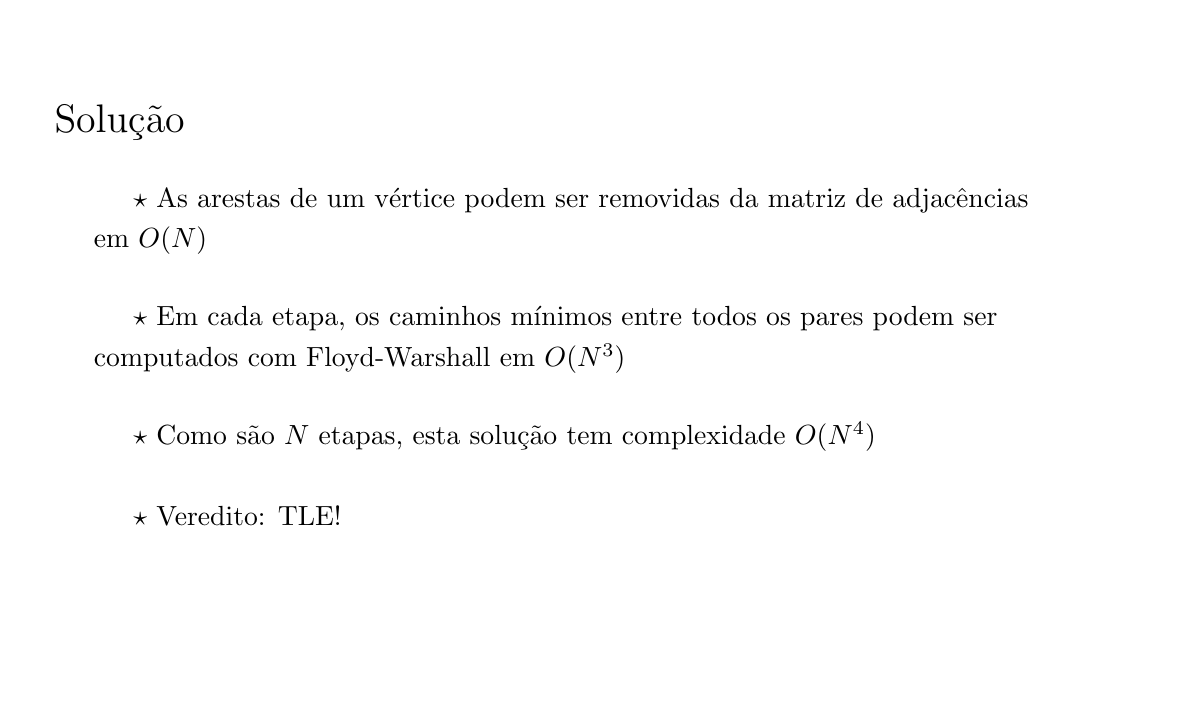
\begin{tikzpicture}
\node[draw,opacity=0] at (0, 0) {x};
\node[draw,opacity=0] at (14, 8) {x};

	\node[anchor=west] (header) at (0.0, 7.0) { \Large \bbbold{Solução} };


	\node[anchor=west] (line1) at (1.0, 6.0) { $\star$ \bbtext{As arestas de um vértice podem ser removidas da matriz de adjacências} };

	\node[anchor=west] (line1a) at (0.5, 5.5) { \bbtext{em $O(N)$} };


	\node[anchor=west] (line2) at (1.0, 4.5) { $\star$ \bbtext{Em cada etapa, os caminhos mínimos entre todos os pares podem ser} };

	\node[anchor=west] (line2a) at (0.5, 4.0) { \bbtext{computados com Floyd-Warshall em $O(N^3)$} };


	\node[anchor=west] (line3) at (1.0, 3.0) { $\star$ \bbtext{Como são $N$ etapas, esta solução tem complexidade $O(N^4)$} };

	\node[anchor=west] (line4) at (1.0, 2.0) { $\star$ \bbbold{Veredito}\bbtext{: TLE!} };

\end{tikzpicture}
\end{frame}
\begin{frame}[plain,t]
\begin{tikzpicture}
\node[draw,opacity=0] at (0, 0) {x};
\node[draw,opacity=0] at (14, 8) {x};

	\node[anchor=west] (header) at (0.0, 7.0) { \Large \bbbold{Solução} };

\end{tikzpicture}
\end{frame}
\begin{frame}[plain,t]
\begin{tikzpicture}
\node[draw,opacity=0] at (0, 0) {x};
\node[draw,opacity=0] at (14, 8) {x};

	\node[anchor=west] (header) at (0.0, 7.0) { \Large \bbbold{Solução} };


	\node[anchor=west] (line1) at (1.0, 6.0) { $\star$ \bbtext{Para reduzir a complexidade, é preciso compreender o funcionamento do} };

	\node[anchor=west] (line1a) at (0.5, 5.5) { \bbtext{algoritmo de Floyd-Warshall} };

\end{tikzpicture}
\end{frame}
\begin{frame}[plain,t]
\begin{tikzpicture}
\node[draw,opacity=0] at (0, 0) {x};
\node[draw,opacity=0] at (14, 8) {x};

	\node[anchor=west] (header) at (0.0, 7.0) { \Large \bbbold{Solução} };


	\node[anchor=west] (line1) at (1.0, 6.0) { $\star$ \bbtext{Para reduzir a complexidade, é preciso compreender o funcionamento do} };

	\node[anchor=west] (line1a) at (0.5, 5.5) { \bbtext{algoritmo de Floyd-Warshall} };


	\node[anchor=west] (line2) at (1.0, 4.5) { $\star$ \bbtext{A cada iteração, as distâncias são relaxadas usando o vértice $k$ como} };

	\node[anchor=west] (line2a) at (0.5, 4.0) { \bbtext{intermediário} };

\end{tikzpicture}
\end{frame}
\begin{frame}[plain,t]
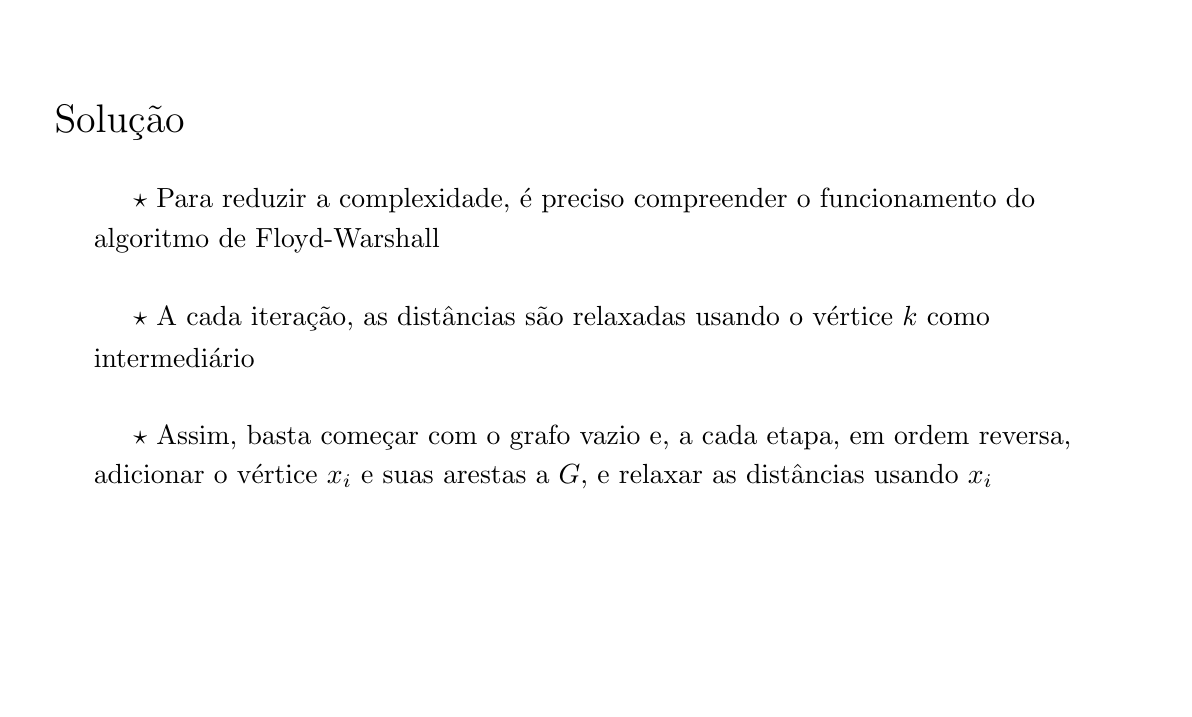
\begin{tikzpicture}
\node[draw,opacity=0] at (0, 0) {x};
\node[draw,opacity=0] at (14, 8) {x};

	\node[anchor=west] (header) at (0.0, 7.0) { \Large \bbbold{Solução} };


	\node[anchor=west] (line1) at (1.0, 6.0) { $\star$ \bbtext{Para reduzir a complexidade, é preciso compreender o funcionamento do} };

	\node[anchor=west] (line1a) at (0.5, 5.5) { \bbtext{algoritmo de Floyd-Warshall} };


	\node[anchor=west] (line2) at (1.0, 4.5) { $\star$ \bbtext{A cada iteração, as distâncias são relaxadas usando o vértice $k$ como} };

	\node[anchor=west] (line2a) at (0.5, 4.0) { \bbtext{intermediário} };


	\node[anchor=west] (line3) at (1.0, 3.0) { $\star$ \bbtext{Assim, basta começar com o grafo vazio e, a cada etapa, em ordem reversa,} };

	\node[anchor=west] (line3a) at (0.5, 2.5) { \bbtext{adicionar o vértice $x_i$ e suas arestas a $G$, e relaxar as distâncias usando $x_i$} };

\end{tikzpicture}
\end{frame}
\begin{frame}[plain,t]
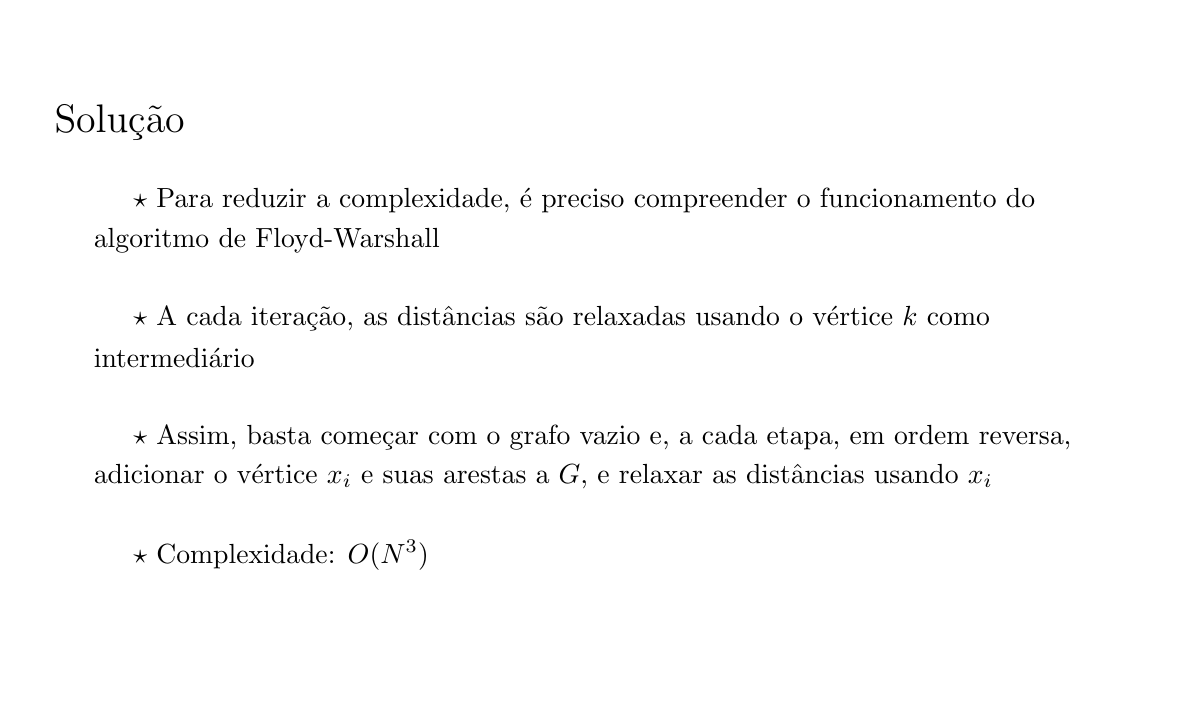
\begin{tikzpicture}
\node[draw,opacity=0] at (0, 0) {x};
\node[draw,opacity=0] at (14, 8) {x};

	\node[anchor=west] (header) at (0.0, 7.0) { \Large \bbbold{Solução} };


	\node[anchor=west] (line1) at (1.0, 6.0) { $\star$ \bbtext{Para reduzir a complexidade, é preciso compreender o funcionamento do} };

	\node[anchor=west] (line1a) at (0.5, 5.5) { \bbtext{algoritmo de Floyd-Warshall} };


	\node[anchor=west] (line2) at (1.0, 4.5) { $\star$ \bbtext{A cada iteração, as distâncias são relaxadas usando o vértice $k$ como} };

	\node[anchor=west] (line2a) at (0.5, 4.0) { \bbtext{intermediário} };


	\node[anchor=west] (line3) at (1.0, 3.0) { $\star$ \bbtext{Assim, basta começar com o grafo vazio e, a cada etapa, em ordem reversa,} };

	\node[anchor=west] (line3a) at (0.5, 2.5) { \bbtext{adicionar o vértice $x_i$ e suas arestas a $G$, e relaxar as distâncias usando $x_i$} };


	\node[anchor=west] (line4) at (1.0, 1.5) { $\star$ \bbbold{Complexidade}\bbtext{: $O(N^3)$} };


\end{tikzpicture}
\end{frame}
\begin{frame}[plain,t]

\inputsnippet{cpp}{11}{28}{codes/10171.cpp}

\end{frame}
\begin{frame}[plain,t]

\inputsnippet{cpp}{30}{42}{codes/10171.cpp}

\end{frame}
\end{document}
